\section{MSSM neutral Higgs production processes\footnote{M.~Spira,
M.~Vazquez Acosta, M.~Warsinsky, G.~Weiglein (eds.); S.~Dittmaier,
R.~Harlander, S.~Heinemeyer, A.~Kalinowski, M.~M\"uhlleitner,
M.~Kr\"amer, H.~Rzehak, M.~Schumacher, P.~Slavich and T.~Vickey.}}
%        =======================================

\label{sec:mssm_neutral}

%\vskip 0.8cm

%\noindent
%{\sc S.~Dittmaier$^1$, R.~Harlander$^2$, S.~Heinemeyer$^3$,
%A.~Kalinowski$^4$, M.~M\"uhlleitner$^5$, M.~Kr\"amer$^6$, H.~Rzehak$^5$,
%M.~Schumacher$^1$, P.~Slavich$^7$, M.~Spira$^8$, M.~Vazquez Acosta$^9$,
%T.~Vickey$^{10}$, M.~Warsinsky$^1$ and G.~Weiglein$^{11}$}

%\vskip 0.8cm

%\begin{small}
%\noindent
%{\it \small
%$^1$ Physikalisches Institut, Albert-Ludwigs-Universit\"at Freiburg,
%D--79104 Freiburg, Germany \\
%$^2$ Bergische Universit\"at Wuppertal, D--42097 Wuppertal, Germany \\
%$^3$ Instituto de F\'isica de Cantabria (CSIC-UC), Santander, Spain \\
%$^4$ Faculty of Physics, University of Warsaw, Hoza 69, 00-681
%Warsaw, Poland \\
%$^5$ Institut f\"ur Theoretische Physik, KIT, D--76128 Karlsruhe, Germany \\
%$^6$ Institut f\"ur Theoretische Physik, RWTH Aachen University,
%D--52056 Aachen, Germany \\
%$^7$ LPTHE, F--75252 Paris, France\\
%$^8$ Paul Scherrer Institut, CH--5232 Villigen PSI, Switzerland \\
%$^9$ Imperial College, University of London, London, United Kingdom \\
%$^{10}$ Oxford University, Department of Physics, Denys Wilkinson Building,
%Keble Road, Oxford OX1 3RH, United Kingdom \\
%$^{11}$ Deutsches Elektronen-Synchrotron, D--22603 Hamburg, Germany}
%\end{small}

%\vskip 0.8cm

\providecommand{\PA}{\mathrm{A}}
\newcommand{\orderx}[1]{\ensuremath{{\cal O}(#1)}}
\newcommand{\mhmaxx}{\ensuremath{m_h^{\rm max}}}
%\newcommand{\gsim}
%{\;\raisebox{-.3em}{$\stackrel{\displaystyle >}{\sim}$}\;}
%\newcommand{\cp}{{\cal CP}}
\newcommand{\cp}{\mathrm{CP}}
\newcommand{\MHp}{M_{\PSHpm}}
\providecommand{\lsim}
{\;\raisebox{-.3em}{$\stackrel{\displaystyle <}{\sim}$}\;}
\providecommand{\gsim}
{\;\raisebox{-.3em}{$\stackrel{\displaystyle >}{\sim}$}\;}
\providecommand{\gghnnlo}{{\sc ggH@NNLO}}
\providecommand{\bbhnnlo}{{\sc bbH@NNLO}}
\providecommand{\HDECAY}{{\sc HDECAY}}
\providecommand{\HIGLU}{{\sc HIGLU}}
\providecommand{\Prophecy}{{\sc Prophecy4f}}
\providecommand{\CPsuperH}{{\sc CPsuperH}}
\providecommand{\FeynHiggs}{{\sc FeynHiggs}}
%\providecommand{\alphas}{\alpha_s}

\subsection{Higgs phenomenology in the MSSM}
\label{sec:mssmvssm}

The Higgs sector of the Minimal Supersymmetric Standard Model (MSSM)
with two scalar doublets accommodates five physical Higgs bosons. In
lowest order these are the light and heavy CP-even $\PSh$ and $\PH$, the
$\cp$-odd $\PSA$, and the charged Higgs bosons $\PSHpm$.  The MSSM Higgs
sector can be expressed at lowest order in terms of the gauge couplings
and two further input parameters, conventionally chosen as $\tanb \equiv
v_2/v_1$, the ratio of the two vacuum expectation values, and either
$\MA$ or $M_{\PSHpm}$. All other masses and mixing angles can therefore be
predicted. However, the Higgs sector of the MSSM is affected by large
higher-order corrections, which have to be taken into account for
reliable phenomenological predictions. In particular, owing to the large
top Yukawa coupling, loop contributions from the top and stop sector to
the Higgs masses and couplings can be numerically very important. For
large values of $\tanb$ also effects from the bottom/sbottom sector can
be large. The relation between the bottom-quark mass and the bottom
Yukawa coupling is affected by a $\tanb$-enhanced contribution
$\Delta_{\PQb}$~\cite{Hall:1993gn,Hempfling:1993kv,
Carena:1994bv,Pierce:1996zz,Carena:1999py,Guasch:2003cv,Noth:2008tw,Noth:2010jy,Mihaila:2010mp,Hofer:2009xb}, which is
non-vanishing even in the limit of asymptotically large values of the
SUSY mass parameters (an analogous contribution also exists for the
$\PGt$ lepton).  While the MSSM Higgs sector is CP-conserving at lowest
order, CP-violating effects can enter via the potentially large loop
corrections, giving rise to a mixing between all three neutral mass
eigenstates. In the following we will focus on the CP-conserving case
and use $\MA$ as input parameter. 

Higgs phenomenology in the MSSM can differ very significantly from the
SM case. The relevant couplings entering production and decay processes
of an MSSM Higgs boson can be much different from the corresponding
couplings in the SM case. The lower bound on the Higgs mass in the SM
from the searches at LEP cannot directly be applied to the MSSM
case~\cite{Barate:2003sz,Schael:2006cr}, and in fact much lighter Higgs 
masses are possible in the MSSM without being in conflict with the
present search limits. The presence of more than one Higgs boson in the
spectrum can give rise to overlapping signals in the Higgs searches, in 
particular in parameter regions where the Higgs-boson widths are large.
On the other hand, 
in the decoupling limit, $\MA \gg \MZ$ (in practice realised already for 
$\MA \gsim 2 \MZ$), the couplings of the light CP-even Higgs boson 
to gauge bosons and fermions become SM-like. In this parameter region 
the light CP-even Higgs boson of the MSSM resembles the 
Higgs boson of the SM. In addition to the production and decay processes 
present for a SM Higgs, further channels are possible in the MSSM case. 
In particular, MSSM Higgs bosons can be produced in association with or
in decays of SUSY particles, and decays of MSSM Higgs bosons into SUSY
particles, if kinematically allowed, can have a large impact on 
the Higgs branching ratios. In some parameter regions even decays of 
heavy MSSM Higgs bosons into lighter Higgs states can be relevant, 
which if detectable could be of great interest to gain information on 
the Higgs self-couplings. In the following we will mainly focus on the 
production processes that are expected to be most relevant for early
searches for MSSM Higgs bosons at the LHC, namely Higgs production in
gluon fusion and in association with bottom quarks.

It is customary to discuss searches for MSSM Higgs bosons in terms of 
benchmark scenarios where the lowest-order input parameters 
$\tanb$ and $\MA$ (or $\MHp$) are varied, while the other SUSY parameters
entering via radiative corrections are set to certain benchmark values. 
In the following we will focus on the $\mhmaxx$ benchmark 
scenario~\cite{Carena:2002qg}, which in the on-shell scheme is defined as
\begin{equation}
M_{\mathrm{SUSY}} = 1 \UTeV, \; X_{\PQt} = 2 M_{\mathrm{SUSY}}, \; \mu = 200 \UGeV, \;
M_{\PSg}=800 \UGeV, \; M_2 = 200 \UGeV, \; A_{\PQb} = A_{\PQt},
\label{YRHXS_MSSM_neutral_eq:mhmax}
\end{equation}
where $M_{SUSY}$ denotes the common soft-SUSY-breaking squark mass of
the third generation, $X_{\PQt}=A_{\PQt}-\mu/\tanb$ the stop mixing
parameter, $A_\mathrm{t}$ and $A_\mathrm{b}$ the stop and sbottom
trilinear couplings, respectively, $\mu$ the Higgsino mass parameter,
$M_{\PSg}$ the gluino mass, and $M_2$ the SU(2)-gaugino mass parameter.
$M_1$ is fixed via the GUT-relation $M_1 = 5/3 M_2 \sin \theta_w/\cos
\theta_w$.

In contrast to the SM case, where the Higgs mass is a free input
parameter, calculations of Higgs-boson production and decay processes in
the MSSM require as a first step the evaluation of the Higgs-boson
masses and mixing contributions in terms of $\MA$, $\tanb$, and all other
SUSY parameters that enter via radiative corrections. The mixing between
the CP-even states $\PSh$ and $\PSH$ (in the approximation where
CP-violating effects are neglected; in general mixing between $\PSh$,
$\PSH$, and $\PSA$ has to be considered) must be taken into account
correctly in order to ensure the correct on-shell properties of the
Higgs fields appearing in the $S$-matrix elements of Higgs-boson
production or decay processes. 

Two dedicated codes exist for calculating the Higgs-boson masses and
mixing contributions in terms of the MSSM input parameters,
\FeynHiggs~\cite{Heinemeyer:1998yj,Heinemeyer:1998np,Degrassi:2002fi,
Frank:2006yh} and \CPsuperH~\cite{Lee:2003nta,Lee:2007gn}, which
incorporate higher-order corrections in the MSSM Higgs sector up to the
two-loop level. In the case of real parameters a more complete set of
higher-order corrections is included in \FeynHiggs. We will therefore
use \FeynHiggs\ for evaluating the Higgs-boson masses and effective
couplings in the MSSM. We have performed a comparison between the
predictions of \FeynHiggs\ and \CPsuperH\ (using an appropriate
parameter transformation to take account of the different
renormalization schemes used in the calculations incorporated in the two
codes) in the $\mhmaxx$ and no-mixing benchmark
scenarios~\cite{Carena:2002qg,Carena:2000dp}. We have found in general
good agreement, with deviations in the prediction of the lightest MSSM
Higgs mass, $\Mh$, of \orderx{1}\UGeV, and deviations of up to $\sim
10\%$ in the effective mixing angle of the neutral $\cp$-even Higgs
sector for large values of $\tanb$.  The deviations can nevertheless be
relevant in the parameter regions that are tested first by the LHC:
relatively low $\MA$ and large $\tanb$.  A numerical comparison of
\FeynHiggs\ and \CPsuperH\ with the program
\HDECAY~\cite{Djouadi:1997yw,Spira:1997dg,hdecay2}, which
performs the calculation of Higgs-boson masses and mixings in the MSSM
using a less complete set of higher-order corrections, is in progress.

In making predictions for Higgs-boson production or decay processes in the MSSM 
one has to face the fact that certain types of higher-order 
corrections have only been calculated in the SM case up to now, while
their counterpart for the case of the MSSM is not yet available. Instead
of starting from dedicated MSSM calculations for Higgs cross sections or
decay widths,  
which treat higher-order corrections of SM-type and SUSY-type on the 
same footing but may be lacking the most up-to-date SM-type corrections,
it can be advantageous to start from SM-type processes including the 
relevant higher-order corrections and to dress suitable building blocks
with appropriate MSSM coupling factors (using also the MSSM predictions
for the Higgs masses). For the numerical results presented below 
on MSSM Higgs production in gluon fusion and in association with bottom
quarks we have followed the latter approach, as explained in more detail
below.


%%%%%%%%%%%%%%%%%%%%%%%%%%%%%%%%%%%%%%%%%%%%%%%%%%%%%%%%%%%%%%%%%%%%%%%%%

\subsection{Overview about the most relevant MSSM Higgs production processes}

The dominant neutral MSSM Higgs production mechanisms for small and
moderate values of $\tan\beta$ are the gluon-fusion processes (see
\Fref{YRHXS_MSSM_neutral_dia1})
\begin{displaymath}
\Pg\Pg \to \PSh,\PSH,\PSA
\end{displaymath}
\begin{figure}[hbt]
\begin{center}
\SetScale{0.8}
\begin{picture}(180,80)(0,0)
\Gluon(0,20)(50,20){-3}{5}
\Gluon(0,80)(50,80){3}{5}
\ArrowLine(50,20)(50,80)
\ArrowLine(50,80)(100,50)
\ArrowLine(100,50)(50,20)
\DashLine(100,50)(150,50){5}
\Vertex(50,20){2}
\Vertex(50,80){2}
\Vertex(100,50){2}
\put(126,37){$\PSh,\PSH,\PSA$}
\put(0,37){$\PQt,\PQb,\PSQt, \PSQb$}
\put(-12,14){$\Pg$}
\put(-12,62){$\Pg$}
\end{picture}  \\
\caption{\label{YRHXS_MSSM_neutral_dia1} Typical diagram
contributing to $\Pg\Pg\to \PSh,\PSH,\PSA$ at lowest order.}
\end{center}
\end{figure}
which are mediated predominantly by top and bottom loops as in the SM
case, but in addition by stop and sbottom loops for the scalar Higgs
bosons $\PSh,\PSH$, if the squarks are light \cite{Dawson:1996xz}. The
NLO QCD corrections to the quark loops are known in the heavy-quark
limit \cite{Djouadi:1991tka,Dawson:1991zj,Kauffman:1993nv,Dawson:1993qf}
as well as including the full quark mass dependence
\cite{Graudenz:1992pv,Spira:1993bb,Spira:1995rr,Harlander:2005rq,
Anastasiou:2006hc,Aglietti:2006tp,Bonciani:2007ex}. They increase the
cross sections by up to about $100\%$ for smaller $\tanb$ and up to about
$50\%$ for large $\tanb$, where the bottom loop contributions become
dominant due to the strongly enhanced bottom Yukawa couplings (for the
light CP-even Higgs this enhancement is only present away from the
decoupling limit, i.e.\ for relatively small $\MA$).  The limit of heavy
quarks is only applicable for $\tanb\lesssim 5$ within about $20{-}25\%$,
if the full mass dependence of the LO terms is taken into account
\cite{Kramer:1996iq,Spira:1997dg,Djouadi:2005gi,Djouadi:2005gj}. Thus
the available NNLO QCD corrections in the heavy-quark limit
\cite{Harlander:2002wh,Harlander:2002vv,
Anastasiou:2002yz,Anastasiou:2002wq,Ravindran:2003um} can only be used
for small and moderate $\tanb$, while for large $\tanb$ one has to rely
on the NLO results including the full mass dependence
\cite{Graudenz:1992pv,Spira:1993bb,Spira:1995rr,
Anastasiou:2006hc,Aglietti:2006tp,Bonciani:2007ex}. The QCD corrections
to the squark loops are known in the heavy-squark limit
\cite{Dawson:1996xz} and including the full mass dependence
\cite{Muhlleitner:2006wx,Anastasiou:2006hc,
Aglietti:2006tp,Bonciani:2007ex}. The full SUSY QCD corrections have
been obtained in the limit of heavy squarks and gluinos
\cite{Harlander:2003bb,Harlander:2003kf,Harlander:2004tp,
Harlander:2005if,Degrassi:2008zj,Muhlleitner:2008yw,Degrassi:2010eu} and
recently including the full mass dependences, too
\cite{Anastasiou:2008rm,Muhlleitner:2010nm}.  The pure QCD corrections
are of about the same size as those to the quark loops thus rendering
the total $K$-factor of similar size as for the quark loops alone with a
maximal deviation of about $10\%$ \cite{Dawson:1996xz}.  The pure
SUSY QCD corrections are small for small values of $\tanb$
\cite{Harlander:2003bb,Harlander:2003kf,Harlander:2004tp,
Harlander:2005if,Anastasiou:2008rm}. For large values of $\tanb$
sizable corrections arise due to $\tanb$-enhanced corrections
\cite{Muhlleitner:2010nm,Degrassi:2010eu}. The NNLL resummation of the
SM Higgs cross section \cite{Catani:2003zt,Ravindran:2005vv,Moch:2005ky}
can also be applied to the scalar MSSM Higgs cross sections in the
regions where the heavy-quark limit is valid. For the pseudoscalar 
Higgs-boson production the NNLL resummation has not been performed so far.

The vector-boson fusion processes
\cite{Cahn:1983ip,Hikasa:1985ee,Altarelli:1987ue} (see
\Fref{YRHXS_MSSM_neutral_dia2})
\begin{displaymath}
\PQq\PQq\to \PQq\PQq+\PW^*\PW^*/\PZ^*\PZ^*\to \PQq\PQq + \PSh/\PSH
\end{displaymath}
play an important role for the light CP-even Higgs boson $\PSh$ in the
decoupling limit, $\MA \gg \MZ$, where it becomes SM-like, and for the
heavy CP-even Higgs boson $\PSH$ for small $\MA$, where $\PSH$ becomes
SM-like. In the other regions the cross sections are suppressed by the
additional SUSY factors of the Higgs couplings. The NLO and approximate
NNLO QCD corrections to the total cross section and the distributions
can be taken from the SM Higgs case and are small
\cite{Han:1992hr,Figy:2003nv,Berger:2004pca,
Ciccolini:2007jr,Ciccolini:2007ec,Bolzoni:2010xr}. The SUSY QCD
corrections mediated by virtual gluino and squark exchange at the
vertices turned out to be small \cite{Djouadi:1999ht,Hollik:2008xn}. The
SUSY electroweak corrections are typically at the level of $1\%$ with
up to $2{-}4\%$ at the edge of the SUSY exclusion
limits~\cite{Hollik:2008xn}.
\begin{figure}[hbt] 
\begin{center}
\SetScale{0.8}
\begin{picture}(120,90)(0,0)
\ArrowLine(0,0)(50,0)
\ArrowLine(50,0)(100,0)
\ArrowLine(0,100)(50,100) 
\ArrowLine(50,100)(100,100)
\Photon(50,0)(50,50){3}{5}
\Photon(50,50)(50,100){3}{5}
\DashLine(50,50)(100,50){5}
\Vertex(50,100){2}
\Vertex(50,50){2}
\Vertex(50,0){2}
\put(87,37){$\PSh,\PSH$}
\put(-12,-2){$\PQq$}
\put(-12,78){$\PQq$}
\put(87,-2){$\PQq$}
\put(87,78){$\PQq$}
\put(44,17){$\PW,\PZ$}
\put(44,57){$\PW,\PZ$}
\end{picture}  \\
\caption{\label{YRHXS_MSSM_neutral_dia2} Diagram contributing to
$\PQq\PQq \to
\PQq\PQq V^*V^* \to \PQq\PQq + \PSh/\PSH$ ($V=\PW,\PZ$) at lowest order.} 
\end{center}
\end{figure}

Higgs-strahlung off $\PW,\PZ$ gauge bosons
\cite{Glashow:1978ab,Kunszt:1991xk} (see
\Fref{YRHXS_MSSM_neutral_dia3})
\begin{displaymath}
\PQq\PAQq\to \PZ^*/\PW^* \to \PZ/\PW + \PSh/\PSH
\end{displaymath}
is most relevant for SM-like Higgs states. This class of processes
gained renewed attention at the LHC in the context of possible
improvements of jet reconstruction and decomposition
techniques~\cite{Butterworth:2008iy}.
The NLO \cite{Han:1991ia,Spira:1997dg} and NNLO \cite{Brein:2003wg} QCD
corrections can be translated from the SM to the MSSM case, and the SUSY QCD
corrections are small \cite{Djouadi:1999ht}. The SUSY electroweak
corrections are unknown.
\begin{figure}[hbt]
\begin{center}
\SetScale{0.8}
\begin{picture}(160,100)(0,-10)
\ArrowLine(0,100)(50,50)
\ArrowLine(50,50)(0,0)
\Photon(50,50)(100,50){3}{5}
\Photon(100,50)(150,100){3}{6}
\DashLine(100,50)(150,0){5}
\Vertex(50,50){2}
\Vertex(100,50){2}
\put(126,-4){$\PSh,\PSH$}
\put(-12,-2){$\PAQq$}
\put(-12,78){$\PQq$}
\put(50,50){$\PW,\PZ$}
\put(126,77){$\PW,\PZ$}
\end{picture}  \\
\caption{\label{YRHXS_MSSM_neutral_dia3} Diagram contributing to
$\PQq\PAQq \to V^* \to V + \PSh/\PSH$ ($V=\PW,\PZ$) at lowest order.}
\end{center}
\end{figure}

Higgs-boson radiation off top quarks
\cite{Raitio:1978pt,Ng:1983jm,Kunszt:1984ri,Gunion:1991kg,Marciano:1991qq}
(see \Fref{YRHXS_MSSM_neutral_dia4})
\begin{displaymath}
\PQq\PAQq/\Pg\Pg\to \PQt\PAQt + \PSh/\PSH/\PSA
\end{displaymath}
plays a significant role at the LHC for the light scalar Higgs particle
only. The NLO QCD corrections are the same as for the SM Higgs boson
with modified top and bottom Yukawa couplings and are thus of moderate
size \cite{Beenakker:2001rj,Beenakker:2002nc,
Reina:2001sf,Dawson:2002tg}. The SUSY QCD corrections have been
computed recently \cite{Peng:2005ti,Hollik:2006vn,
Hafliger:2006zz,Walser:2008zz}. They are of moderate size, too.
\begin{figure}[hbt]
\begin{center}
\SetScale{0.8}
\begin{picture}(360,100)(0,-10)
\ArrowLine(0,100)(50,50)
\ArrowLine(50,50)(0,0)
\Gluon(50,50)(100,50){3}{5}
\ArrowLine(100,50)(125,75)
\ArrowLine(125,75)(150,100)
\ArrowLine(150,0)(100,50)
\DashLine(125,75)(150,50){5}
\Vertex(50,50){2}
\Vertex(100,50){2}
\Vertex(125,75){2}
\put(126,37){$\PSh,\PSH,\PSA$}
\put(-12,78){$\PQq$}
\put(-12,-2){$\PAQq$}
\put(55,52){$\Pg$}
\put(126,78){$\PQt/\PQb$}
\put(126,-2){$\PAQt/\PAQb$}
\Gluon(250,0)(300,0){3}{5}
\Gluon(250,100)(300,100){3}{5}
\ArrowLine(350,0)(300,0)
\ArrowLine(300,0)(300,50)
\ArrowLine(300,50)(300,100)
\ArrowLine(300,100)(350,100)
\DashLine(300,50)(350,50){5}
\Vertex(300,100){2}
\Vertex(300,50){2}
\Vertex(300,0){2}
\put(286,37){$\PSh,\PSH,\PSA$}
\put(190,78){$\Pg$}
\put(190,-2){$\Pg$}
\put(286,78){$\PQt/\PQb$}
\put(286,-2){$\PAQt/\PAQb$}
\end{picture}  \\
\caption{\label{YRHXS_MSSM_neutral_dia4} Typical diagrams contributing to
$\PQq\PAQq/\Pg\Pg \to Q\bar Q + \PSh/\PSH/\PSA~~(Q=\PQt,\PQb)$ at lowest order.}
\end{center}
\end{figure}

For large values of $\tanb$ Higgs-boson radiation off bottom quarks
\cite{Raitio:1978pt,Ng:1983jm,Kunszt:1984ri,Gunion:1991kg,Marciano:1991qq}
(see \Fref{YRHXS_MSSM_neutral_dia4})
\begin{displaymath}
\PQq\PAQq/\Pg\Pg\to \PQb\PAQb + \PSh/\PSH/\PSA
\end{displaymath}
constitute the dominant Higgs-boson production processes. The NLO QCD
corrections can be taken from the analogous calculation involving top
quarks. However, they turn out to be large
\cite{Dittmaier:2003ej,Dawson:2003kb}. The main
reason is that the integration over the transverse momenta of the final-state 
bottom quarks generates large logarithmic contributions. The
resummation of the latter can be established by the introduction of bottom-quark
densities in the proton, since the large logarithms correspond to the
DGLAP evolution of these densities. Their DGLAP evolution resums them.
This leads to an approximate approach starting from the process
\cite{Dicus:1988cx} (see \Fref{YRHXS_MSSM_neutral_dia5}a)
\begin{displaymath}
\PQb\PAQb\to \PSh/\PSH/\PSA
\end{displaymath}
at LO, where the transverse momenta of the incoming bottom quarks, their
masses and their off-shellness are neglected at LO. 
\begin{figure}[htbp]
\begin{center}
\SetScale{0.8}
\begin{picture}(130,90)(10,0)
\ArrowLine(0,0)(50,50)
\ArrowLine(50,50)(0,100)
\DashLine(50,50)(100,50){5}
\Vertex(50,50){2}
\put(-12,-2){$\PAQb$}
\put(-12,78){$\PQb$}
\put(88,36){$\PSh/\PSH/\PSA$}
\put(40,-30){{(a)}}
\end{picture}
\hspace*{2em}
\begin{picture}(130,90)(210,0)
\Gluon(250,0)(300,0){3}{5}
\Gluon(250,100)(300,100){3}{5}
\ArrowLine(350,0)(300,0)
\ArrowLine(300,0)(300,50)
\ArrowLine(300,50)(300,100)
\ArrowLine(300,100)(350,100)
\DashLine(300,50)(350,50){5}
\Vertex(300,100){2}
\Vertex(300,50){2}
\Vertex(300,0){2}
\put(286,36){$\PSh/\PSH/\PSA$}
\put(188,78){$\Pg$}
\put(188,-2){$\Pg$}
\put(286,78){$\PQb$}
\put(286,-2){$\PAQb$}
\put(240,-30){{(b)}}
\end{picture} \\[1.0cm]
\caption{\label{YRHXS_MSSM_neutral_dia5} Typical diagrams for the
Higgs-boson production mechanisms related to Higgs radiation off bottom
quarks in the 5FS and 4FS at leading order: {(a)} $\PQb\PAQb\to
\PSh/\PSH/\PSA$ (5FS) and {(b)} $\Pg\Pg\to \PQb\PAQb+\PSh/\PSH/\PSA$
(4FS).}
\end{center}
\end{figure}
The NLO~\cite{Dicus:1998hs,Balazs:1998sb} and NNLO
\cite{Harlander:2003ai} QCD corrections to these bottom-initiated
processes are known and of moderate size, if the running bottom Yukawa
coupling is introduced at the scale of the corresponding Higgs-boson
mass. At NNLO the full process $\Pg\Pg\to \PQb\PAQb + \PSh/\PSH/\PSA$
(see \Fref{YRHXS_MSSM_neutral_dia5}b) contributes to the real
corrections for the first time.  The fully exclusive $\Pg\Pg\to
\PQb\PAQb + \PSh/\PSH/\PSA$ process, calculated with four active parton
flavours in a four-flavour scheme (4FS), and the result, calculated with
five active parton flavours in the five-flavour scheme (5FS), will converge
against the same value at higher perturbative orders. Reasonable
agreement between the NLO 4FS and NNLO 5FS is achieved if the
factorization scale of the bottom-quark densities is chosen as about a
quarter of the Higgs mass \cite{Campbell:2004pu,Dawson:2005vi}.  If both
bottom jets accompanying the Higgs boson in the final state are tagged,
one has to rely on the fully exclusive calculation for $\Pg\Pg\to
\PQb\PAQb + \PSh/\PSH/\PSA$. For the case of a single $\PQb$-tag in the
final state the corresponding calculation in the 5FS starts from the
process $\PQb\Pg\to \PQb+\PSh/\PSH/\PSA$ with the final-state bottom
quark carrying finite transverse momentum.
The NLO QCD and electroweak corrections to this process have been
calculated \cite{Campbell:2002zm,Dawson:2004sh,Beccaria:2010fg}
supplemented by the NLO SUSY QCD corrections recently \cite{Dawson:2007ur}.


In our study we concentrated on the gluon-fusion processes and neutral
Higgs-boson radiation off bottom quarks as the first step. We have
focused on the $\mhmaxx$ scenario \cite{Carena:2000dp,Carena:2002qg},
which is characterised by rather heavy SUSY particles. Genuine SUSY QCD
and SUSY electroweak corrections in this scenario are below the $10\%$
level for Higgs-boson radiation off bottom quarks as well as the 
gluon-fusion processes.  For the calculation of the MSSM Higgs-boson masses
and couplings we have used the program
\FeynHiggs\,2.7.4~\cite{Heinemeyer:1998yj,Heinemeyer:1998np,Degrassi:2002fi,
Frank:2006yh} which includes the most up-to-date radiative corrections
to the MSSM Higgs sector up to the two-loop level and the
$\Delta_{\PQb}$ terms as an approximation of the SUSY QCD and electroweak
corrections to the bottom Yukawa couplings. In further steps we will
have to include the full SUSY QCD and SUSY electroweak corrections
where available and in addition allow for complex MSSM parameters which
leads to additional complications of the Higgs sector, since the mass
eigenstates will no longer be CP-eigenstates.  Moreover, for this study
we have fixed the MSSM scenario, since otherwise general predictions as
in the SM case will not be possible due to the huge variety of the MSSM
parameter space.  However, the results in the $\mhmaxx$ scenario will
not be representative for all possible MSSM scenarios. In the further
progress of this work we will develop the machinery to be able to cover
as many aspects of the MSSM as possible.  This requires the combination
of the most advanced results and tools available in our HEP community
for neutral MSSM Higgs-boson production.

\subsection{Gluon fusion}
%           ============
The gluon-fusion processes $\Pg\Pg\to\phi~(\phi = \PSh,\PSH,\PSA)$ have been
calculated by generating grids for the individual contributions of the
top and bottom-quark loops. Stop and sbottom loops have been neglected
in this first step but will be included in the next steps. We have
generated grids for the scalar and pseudoscalar Higgs bosons
individually with Yukawa couplings of SM-like strength. The MSSM cross
sections can then be obtained by rescaling the individual parts by the
corresponding MSSM Yukawa coupling factors,
\begin{eqnarray}
\sigma^{\mathrm{MSSM}}(\Pg\Pg\to\phi) & = & \left(\frac{g_{\PQt}^{\mathrm{MSSM}}}{g_{\PQt}^{\mathrm{SM}}}\right)^2
\sigma_{\PQt\PQt}(\Pg\Pg\to\phi) + \left(\frac{g_{\PQb}^{\mathrm{MSSM}}}{g_{\PQb}^{\mathrm{SM}}}\right)^2
\sigma_{\PQb\PQb}(\Pg\Pg\to\phi) \nonumber \\
& & +
\frac{g_{\PQt}^{\mathrm{MSSM}}}{g_{\PQt}^{\mathrm{SM}}}~\frac{g_{\PQb}^{\mathrm{MSSM}}}{g_{\PQb}^{\mathrm{SM}}}
\sigma_{\PQt\PQb}(\Pg\Pg\to\phi),
\label{YRHXS_MSSM_neutral_eq1}
\end{eqnarray}
where $\sigma_{\PQt\PQt}, \sigma_{\PQb\PQb}$, and $\sigma_{\PQt\PQb}$ denote the square of
the top contributions, the square of the bottom contributions, and the
top--bottom interference, respectively. For $\sigma_{\PQb\PQb}$ and
$\sigma_{\PQt\PQb}$ we have used the full NLO QCD calculation of \HIGLU
\cite{Spira:1995mt}. For $\sigma_{\PQt\PQt}$ we have used the full NLO QCD
result of \HIGLU~and added the NNLO corrections in the heavy-top-quark
limit by using the program \gghnnlo~\cite{Harlander:2002wh,Harlander:2002vv} in the following way:
$\sigma^0_{\LO}, \sigma^0_{\NLO}$, and $\sigma^0_{\mathrm{NNLO}}$ have been
calculated by \gghnnlo.  The additional part added to the full NLO
result of $\sigma_{\PQt\PQt}$ is then given by
\begin{eqnarray}
\Delta\sigma^{\mathrm{NNLO}}_{\PQt\PQt}(\Pg\Pg\to\phi) & = & \Delta K_{\mathrm{NNLO}}~
\sigma_{\PQt\PQt}^{\mathrm{LO}}(\Pg\Pg\to\phi), \nonumber \\
\Delta K_{\mathrm{NNLO}} & = & \frac{\sigma^0_{\mathrm{NNLO}}-\sigma^0_{\NLO}}{\sigma^0_{\LO}},
\end{eqnarray}
where the individual cross sections $\sigma^0_{\mathrm{LO}}, \sigma^0_{\NLO},
\sigma^0_{\mathrm{NNLO}}$ have been evaluated consistently with LO, NLO, and NNLO
PDFs, respectively.  Since top mass effects are small at NNLO
\cite{Marzani:2008az,Harlander:2009bw,Harlander:2009mq,Harlander:2009my,
Pak:2009bx,Pak:2009dg} this procedure provides a result that is
expected to be very close to full NNLO QCD accuracy for the
$\sigma_{\PQt\PQt}$ parts.  Electroweak corrections to MSSM Higgs-boson
production via gluon fusion have not been calculated. The corresponding
electroweak corrections in the SM case
\cite{Djouadi:1994ge,Aglietti:2004nj,Degrassi:2004mx,Actis:2008ug}
cannot be translated easily to the MSSM and have thus been neglected.
Moreover, we have neglected the NNLL resummation effects
\cite{Catani:2003zt,Ravindran:2005vv,Moch:2005ky} on the
$\sigma_{\PQt\PQt}$ part for two reasons: (i) The NNLL resummation has not
been calculated for the pseudoscalar Higgs boson so far so that in order
to treat the scalar and pseudoscalar Higgs bosons at the same level, the
NNLL effects should be neglected. (ii) For a completely consistent NNLL
prediction also NNLL PDFs would be needed which, however, are not
available. To use NNLO PDFs instead is not fully consistent.

The top and bottom-quark masses have been introduced as pole masses in
the calculation including the corresponding Yukawa couplings. The MSSM
Yukawa coupling ratios to the SM couplings in
Eq.~(\ref{YRHXS_MSSM_neutral_eq1}) have been taken from the program
\FeynHiggs\,2.7.4~\cite{Heinemeyer:1998yj,Heinemeyer:1998np,Degrassi:2002fi,
Frank:2006yh} . As mentioned above, for the numerical MSSM results we
have chosen the $\mhmaxx$ benchmark scenario as specified in
Eq.~(\ref{YRHXS_MSSM_neutral_eq:mhmax}).  As the central choices of the
renormalization and factorization scales we adopted the corresponding
Higgs-boson mass $M_\phi$. For the NLO pieces of the cross section we
used the NLO MSTW2008 PDFs, while for the NNLO contributions the NNLO
MSTW2008 PDFs have been used appropriately. The strong coupling constant
has been normalized according to the PDFs, i.e.~$\alphas(\MZ)=0.12018$
at NLO and $\alphas(\MZ)=0.11707$ at NNLO
\cite{Martin:2009iq,Martin:2009bu}. The scale uncertainty has been
determined by varying the renormalization and factorization scales
between $M_\phi/2$ and $2M_\phi$. It amounts to about $10{-}15\%$ for the whole
Higgs mass and $\tanb$ range although for large values of $\tanb$ the
results are dominated by the bottom-quark loops which are only known at
NLO, unless the light (heavy) scalar Higgs mass is close to its upper
(lower) bound, where the top loops are dominant for large values of
$\tanb$, too. However, the scale dependence of the bottom-quark
contributions is considerably smaller than that of the top quark ones
\cite{Spira:1993bb,Spira:1995rr}.  We have added the $68\%$
CL~PDF+$\alphas$ uncertainties of the MSTW2008 PDFs to the scale
uncertainties linearly. Since there are no NNLO PDF sets of CTEQ and
NNPDF we did not include those sets in this uncertainty.

We have generated grids of the three cross section parts
$\sigma_{\PQt\PQt}^{\mathrm{NNLO}}, \sigma_{\PQb\PQb}^{\NLO}$, and $\sigma_{\PQt\PQb}^{\NLO}$ for the
mass ranges from $70\UGeV$ up to $1\UTeV$ in steps of $1\UGeV$ for the
scalar and pseudoscalar Higgs bosons separately. These grids are then
used for interpolation and the resulting numbers rescaled and added
according to the coupling ratios of \FeynHiggs. For the $\mhmaxx$ scenario we
have included the $\tanb$-enhanced $\Delta_{\PQb}$ corrections in the
effective MSSM bottom Yukawa couplings, since we expect them to dominate
the full SUSY QCD corrections for squark and gluino masses much larger
than the Higgs masses \cite{Degrassi:2010eu}. The resulting cross
sections for the pseudoscalar Higgs boson are shown for various values
of $\tanb$ in \Fref{YRHXS_MSSM_neutral_fig1}, while
Figs.~\ref{YRHXS_MSSM_neutral_fig2} and \ref{YRHXS_MSSM_neutral_fig3}
display the corresponding results for the light and heavy CP-even MSSM
Higgs bosons. The overall scale and PDF+$\alphas$ uncertainties amount to
about $15\%$. It is visible that for small and moderate values of
$\tanb$ virtual $\PQt\PAQt$ thresholds develop for Higgs masses
$M_\phi=2\Mt$, while for large values of $\tanb$ this threshold
behaviour is strongly suppressed due to the dominance of the bottom-quark 
contributions. For the light CP-even Higgs boson most of the
displayed parameter region corresponds to rather low values of $\MA$ 
(which is the input parameter that has been varied in the plots), while
the decoupling region where $\MA \gg \MZ$ corresponds to the region of
the highest $\Mh$ values in the plots. It should be noted that in this
limit, i.e.\ for the upper bound of the light CP-even Higgs-boson mass
in the plots, the light scalar Higgs-boson 
production cross section approaches the NNLO SM result by
construction. Note that the full MSSM result including stop and
sbottom loop contributions does {\it not} approach the SM cross section
for the light scalar Higgs boson at its upper mass bound in general. The
additional contributions from the stops and sbottoms impose a mismatch
between the MSSM cross section in the decoupling limit and the
corresponding SM cross section. This differs from the results of
Section 2 which include the NNLL resummation effects by less than $10\%$,
i.e.~less than the residual scale uncertainties.
\vspace{1cm}

\begin{figure}[htb]
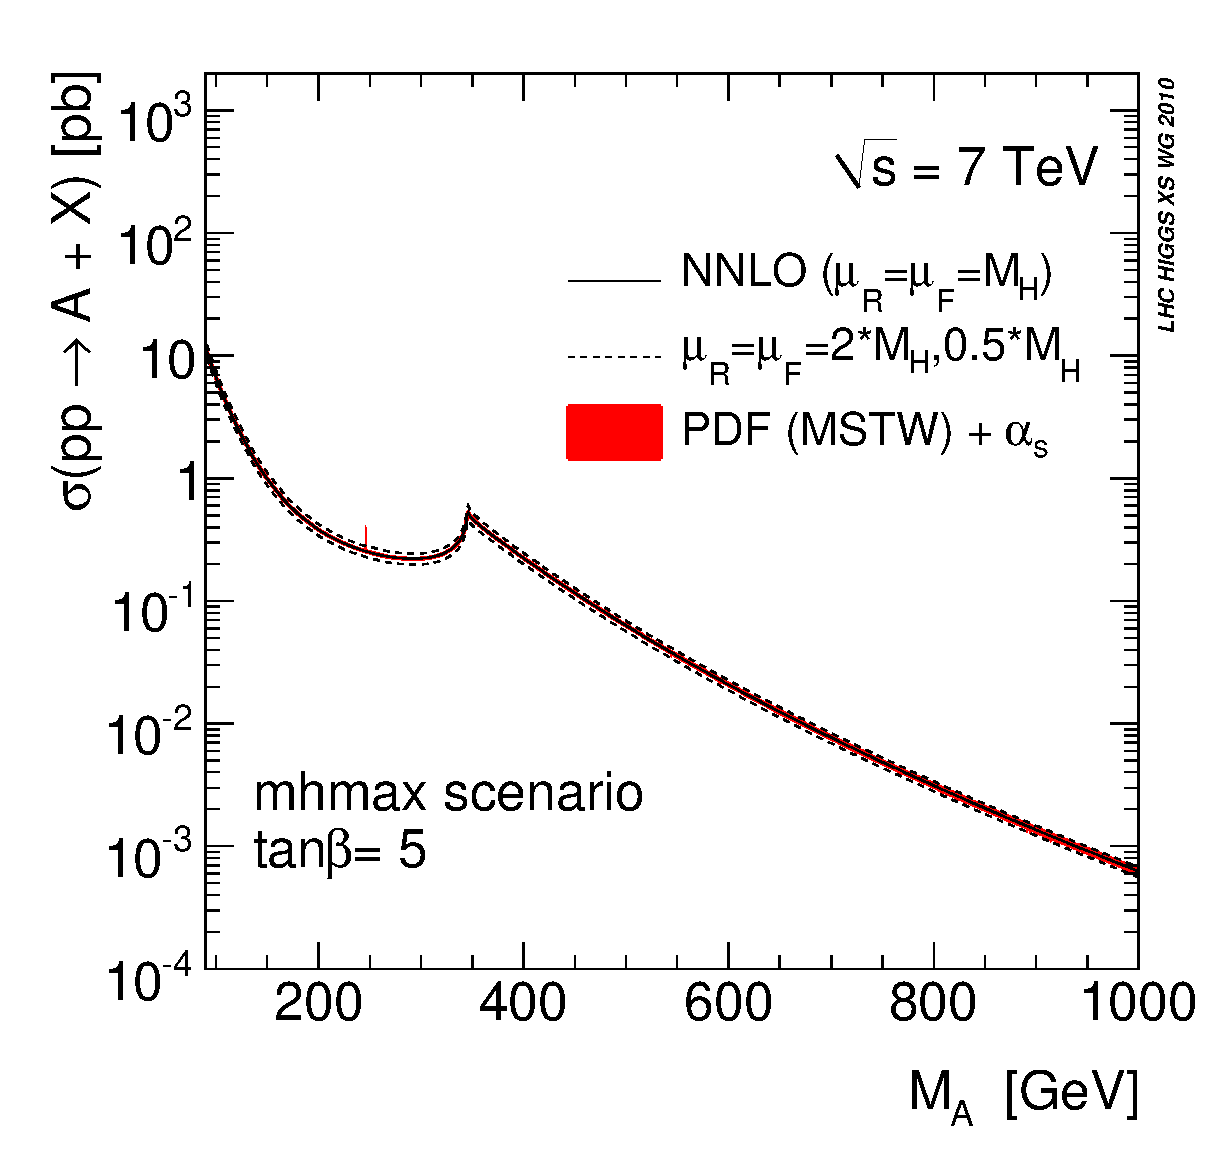
\includegraphics[width=0.5\textwidth]{YRHXS_MSSM_neutral/YRHXS_MSSM_neutral_fig1a.eps}
\includegraphics[width=0.5\textwidth]{YRHXS_MSSM_neutral/YRHXS_MSSM_neutral_fig1b.eps}
\includegraphics[width=0.5\textwidth]{YRHXS_MSSM_neutral/YRHXS_MSSM_neutral_fig1c.eps}
\includegraphics[width=0.5\textwidth]{YRHXS_MSSM_neutral/YRHXS_MSSM_neutral_fig1d.eps}
\caption{\label{YRHXS_MSSM_neutral_fig1} Total gluon-fusion cross
sections of the pseudoscalar MSSM Higgs boson $\PSA$ for four values of
$\tanb$ within the $\mhmaxx$ scenario for $\sqrt{s}=7$\UTeV\ using
MSTW2008 PDFs \cite{Martin:2009iq,Martin:2009bu}. The NNLO results for
the SM-type contributions have been obtained from the programs
\HIGLU~and \gghnnlo, while the rescaling with MSSM coupling factors has
been done with \FeynHiggs.}
\end{figure}

\begin{figure}[htb]
%\begin{picture}(130,200)(30,0)
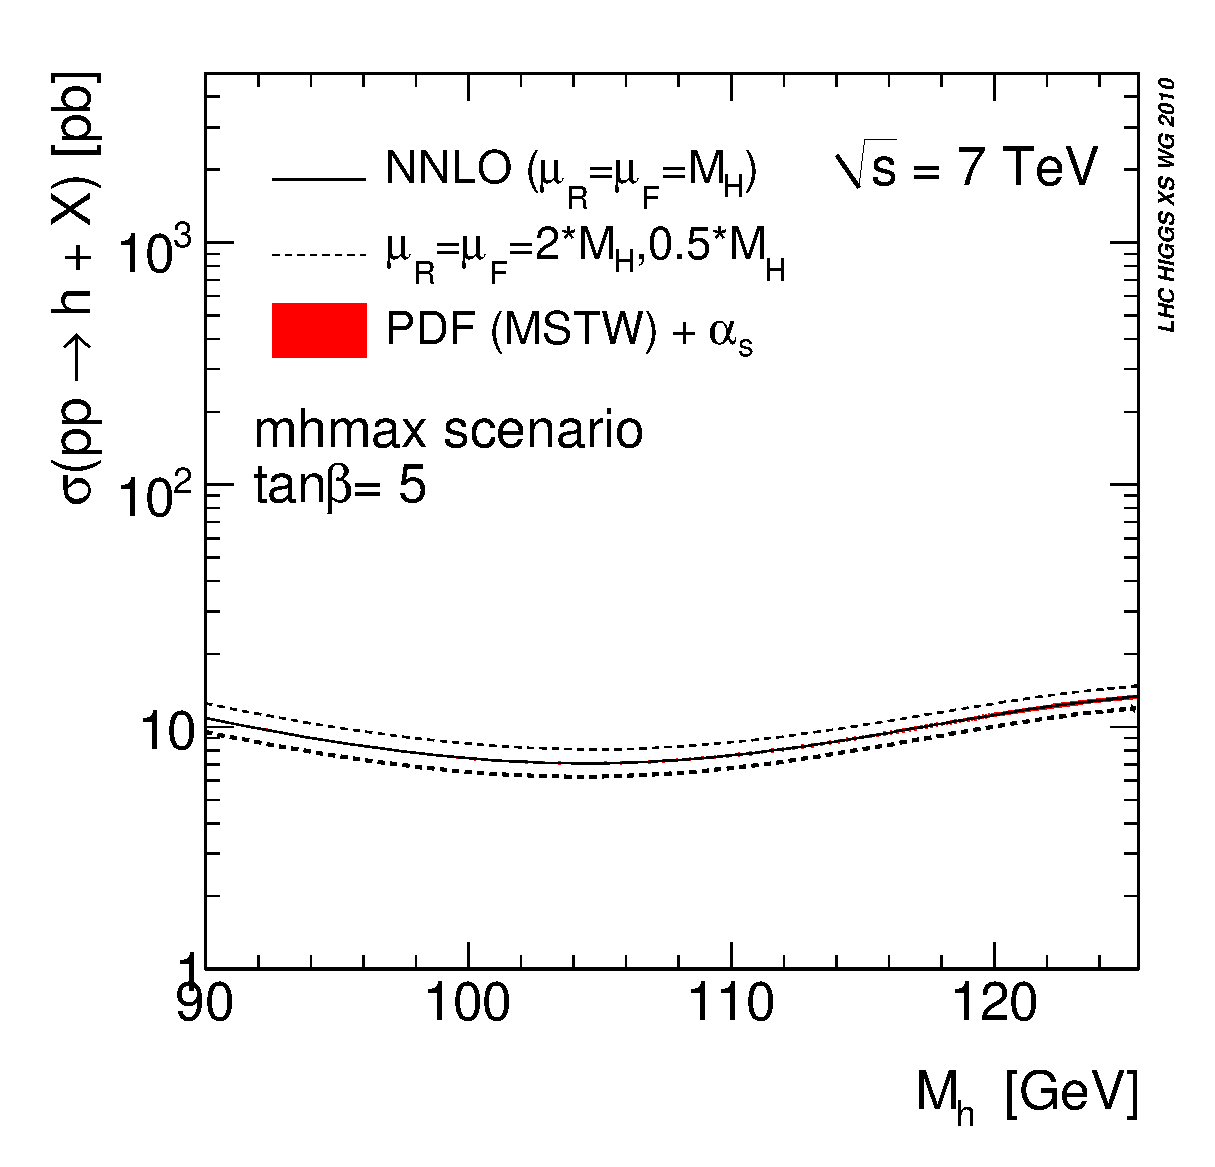
\includegraphics[width=0.5\textwidth]{YRHXS_MSSM_neutral/YRHXS_MSSM_neutral_fig2a.eps}
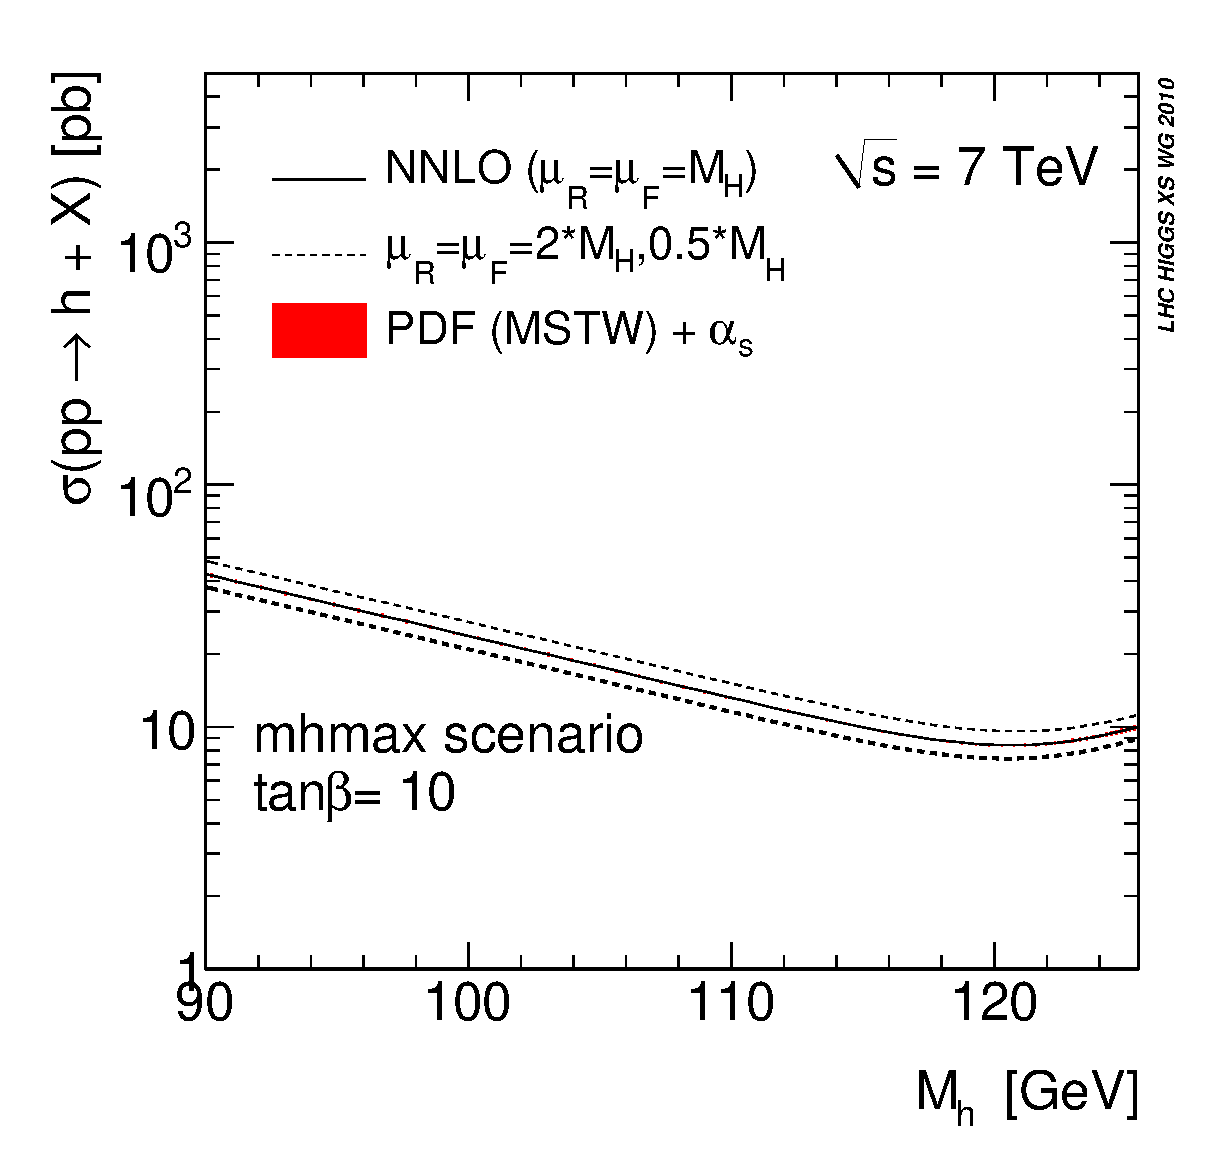
\includegraphics[width=0.5\textwidth]{YRHXS_MSSM_neutral/YRHXS_MSSM_neutral_fig2b.eps}
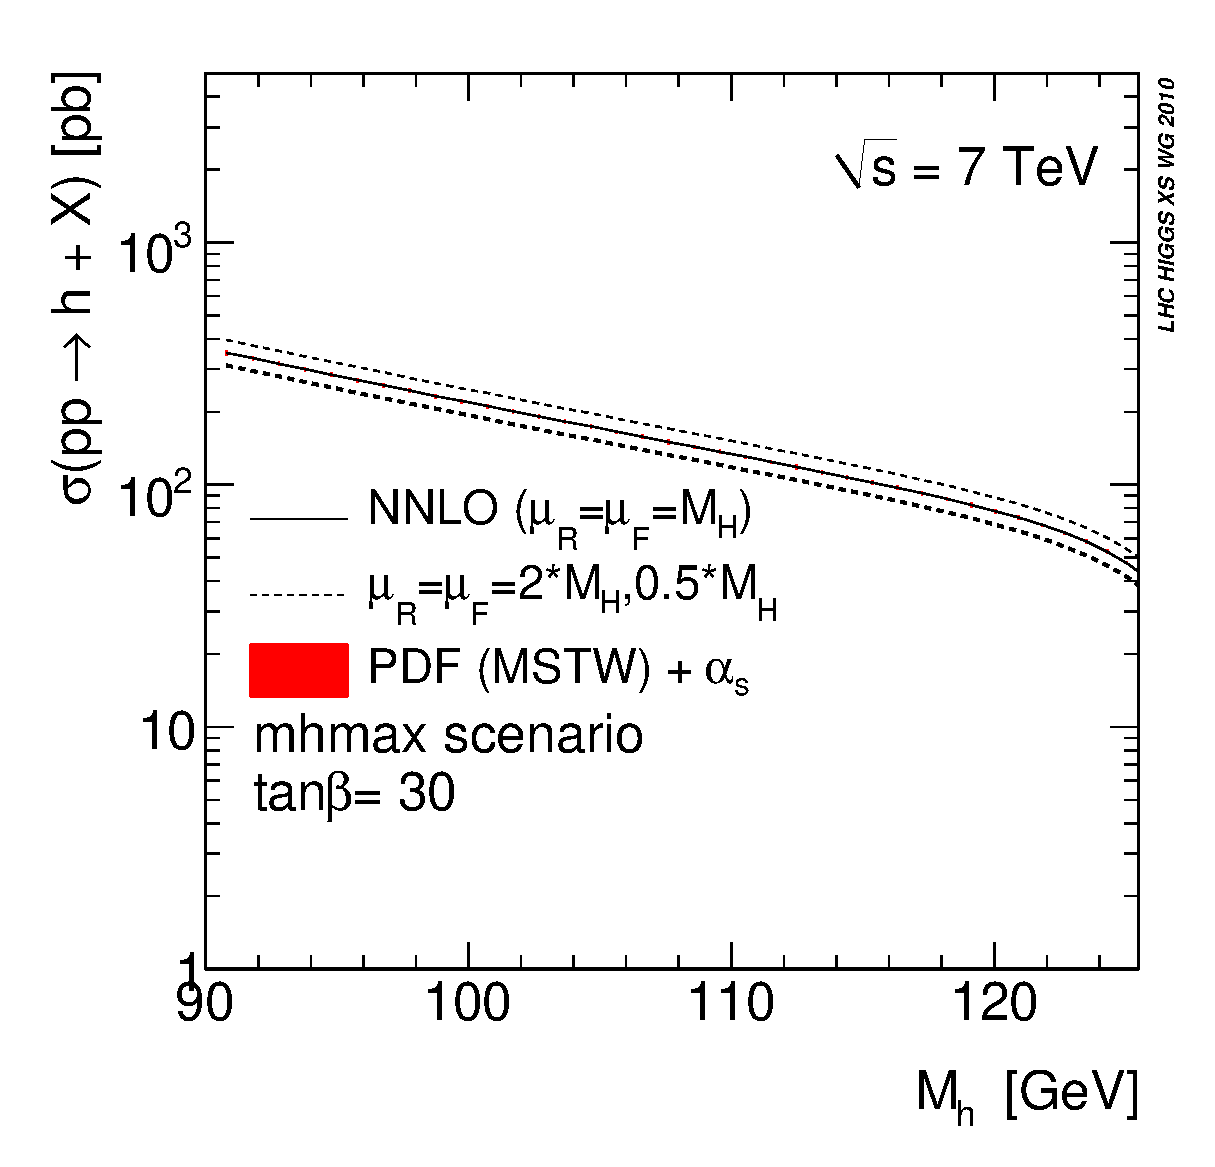
\includegraphics[width=0.5\textwidth]{YRHXS_MSSM_neutral/YRHXS_MSSM_neutral_fig2c.eps}
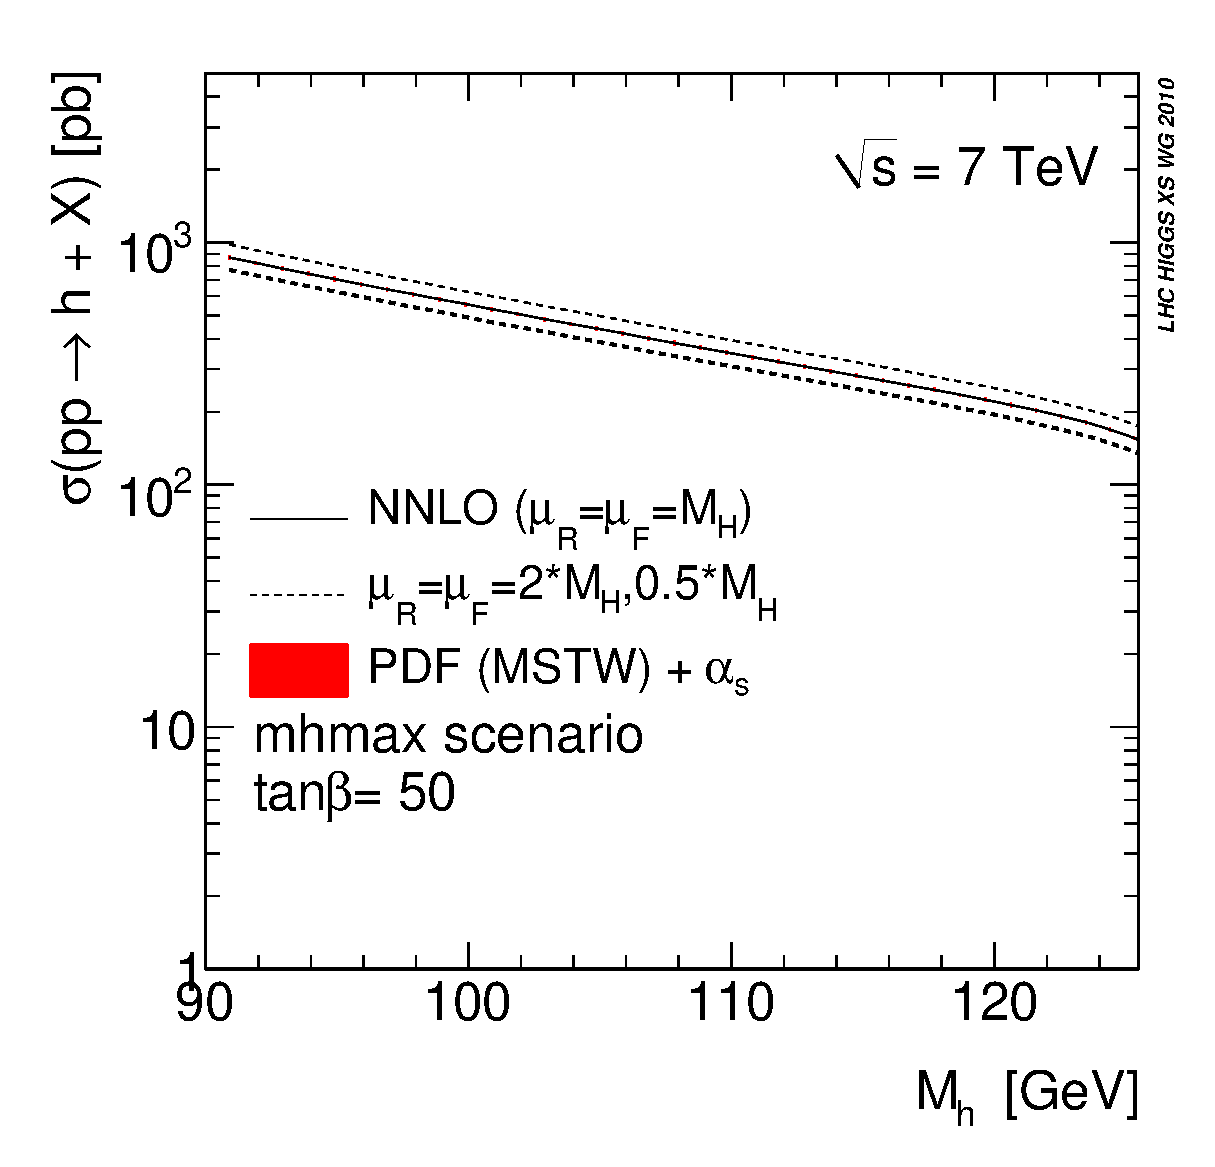
\includegraphics[width=0.5\textwidth]{YRHXS_MSSM_neutral/YRHXS_MSSM_neutral_fig2d.eps}
%\put(30,0){\includegraphics[scale=0.32]{YRHXS_MSSM_neutral/ggl1.eps}}
%\put(270,0){\includegraphics[scale=0.32]{YRHXS_MSSM_neutral/ggl2.eps}}
%\put(30,-220){\includegraphics[scale=0.32]{YRHXS_MSSM_neutral/ggl3.eps}}
%\put(270,-220){\includegraphics[scale=0.32]{YRHXS_MSSM_neutral/ggl4.eps}}
%\end{picture} \\[7.0cm]
\caption{\label{YRHXS_MSSM_neutral_fig2} Total gluon-fusion cross
sections of the light scalar (CP-even) MSSM Higgs boson $\PSh$ for four values of
$\tanb$ within the $\mhmaxx$ scenario for $\sqrt{s}=7$\UTeV\ using
MSTW2008 PDFs \cite{Martin:2009iq,Martin:2009bu}. The NNLO results for
the SM-type contributions have been obtained from the programs
\HIGLU~and \gghnnlo, while the rescaling with MSSM coupling factors has
been done with \FeynHiggs.}

\end{figure}
\begin{figure}[htb]
%\begin{picture}(130,200)(30,0)
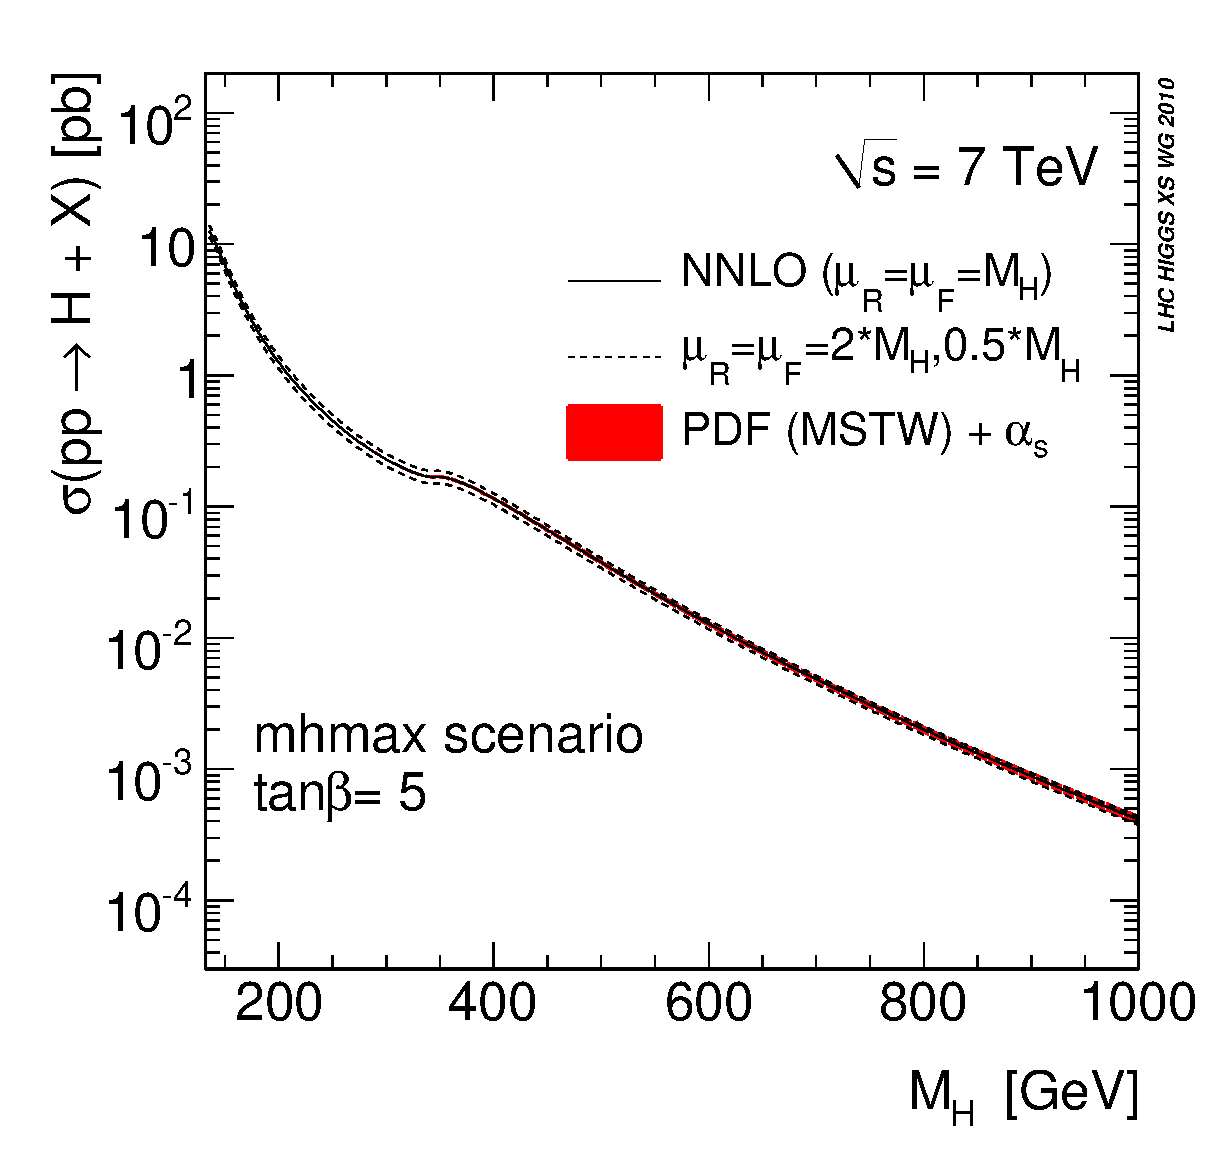
\includegraphics[width=0.5\textwidth]{YRHXS_MSSM_neutral/YRHXS_MSSM_neutral_fig3a.eps}
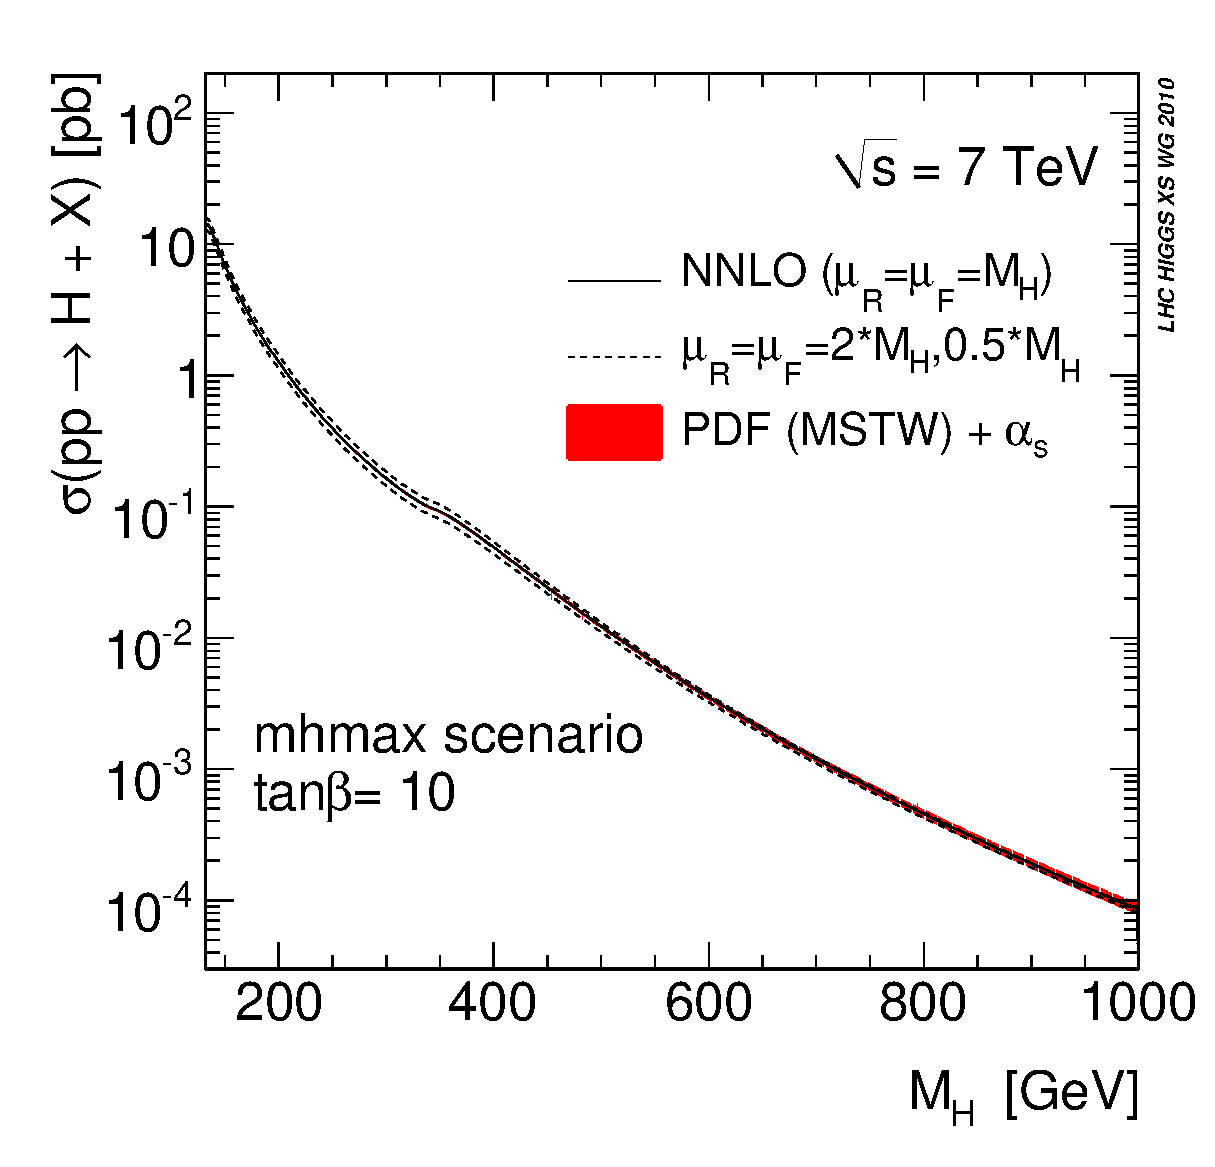
\includegraphics[width=0.5\textwidth]{YRHXS_MSSM_neutral/YRHXS_MSSM_neutral_fig3b.eps}
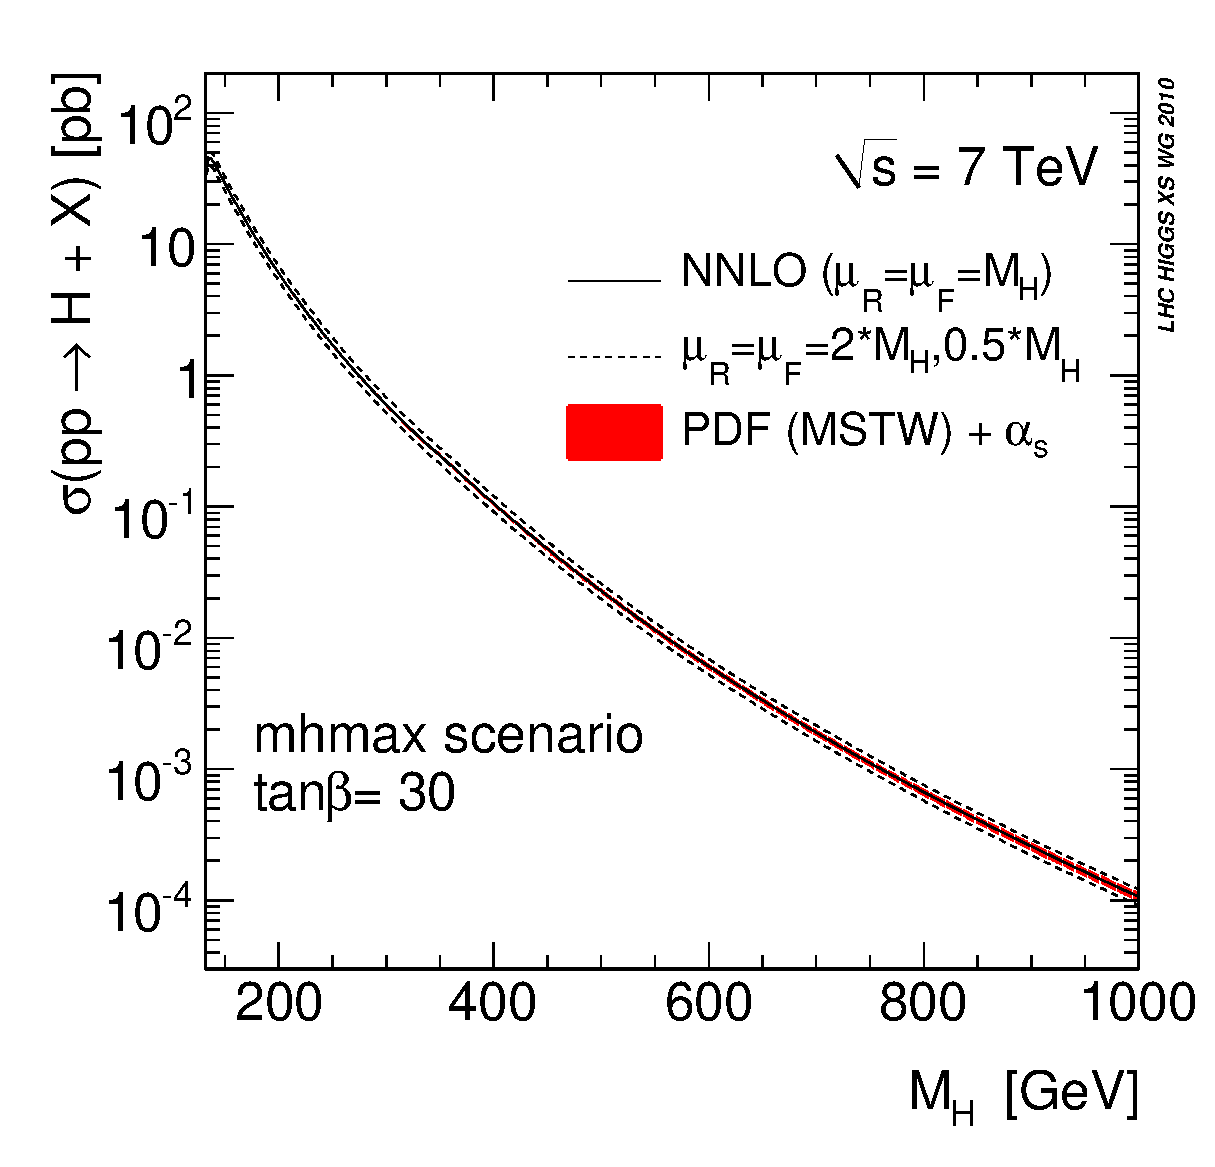
\includegraphics[width=0.5\textwidth]{YRHXS_MSSM_neutral/YRHXS_MSSM_neutral_fig3c.eps}
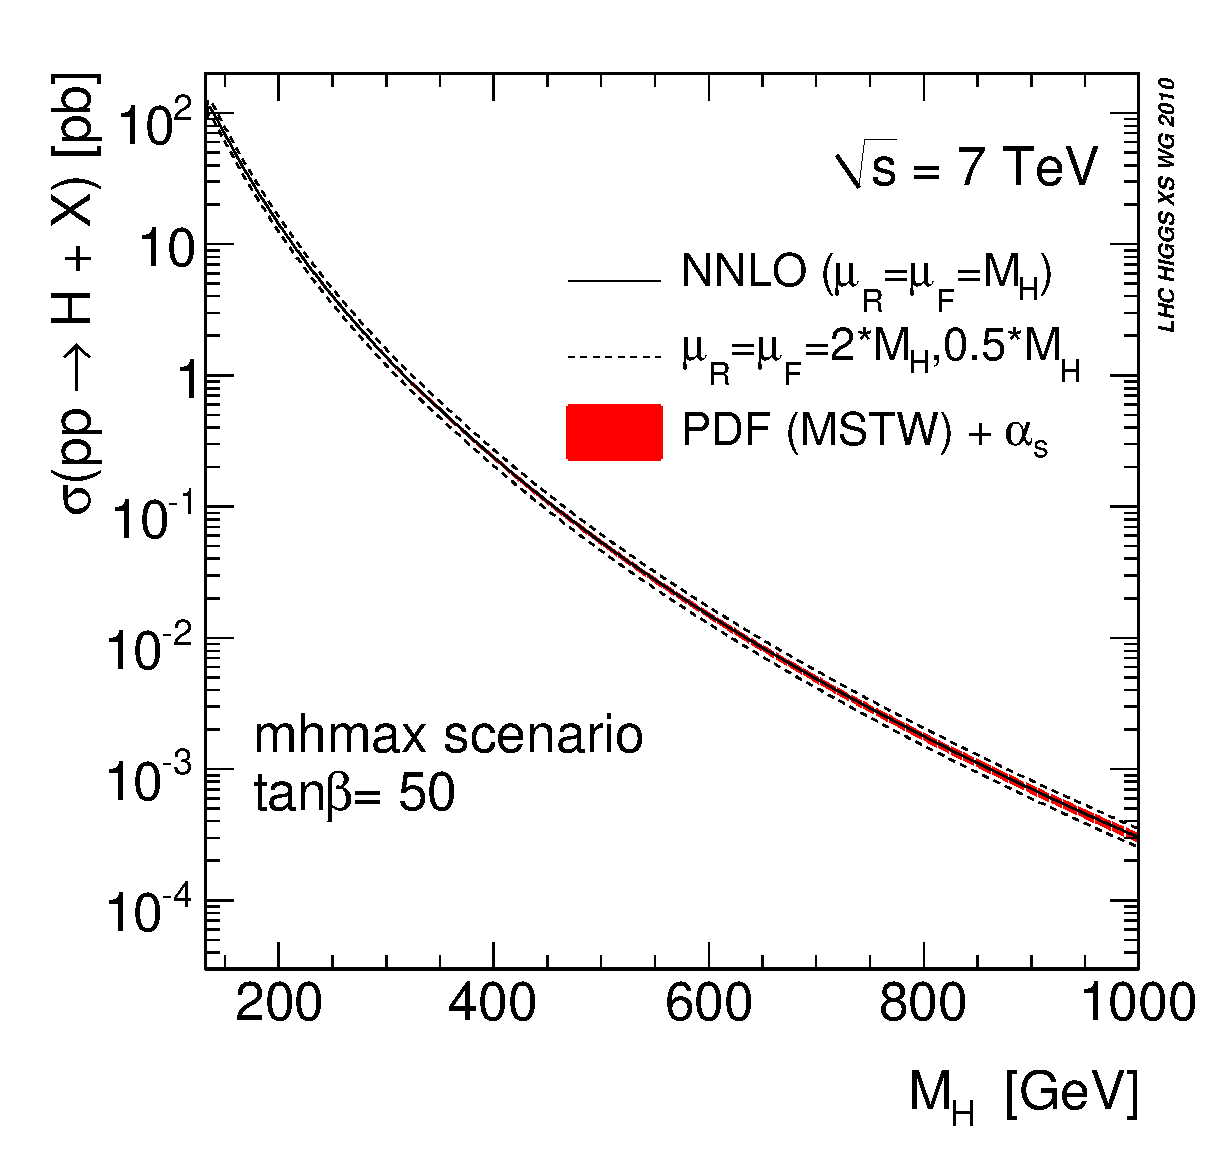
\includegraphics[width=0.5\textwidth]{YRHXS_MSSM_neutral/YRHXS_MSSM_neutral_fig3d.eps}
%\put(30,0){\includegraphics[scale=0.32]{YRHXS_MSSM_neutral/ggh1.eps}}
%\put(270,0){\includegraphics[scale=0.32]{YRHXS_MSSM_neutral/ggh2.eps}}
%\put(30,-220){\includegraphics[scale=0.32]{YRHXS_MSSM_neutral/ggh3.eps}}
%\put(270,-220){\includegraphics[scale=0.32x]{YRHXS_MSSM_neutral/ggh4.eps}}
%\end{picture} \\[7.0cm]
\caption{\label{YRHXS_MSSM_neutral_fig3} Total gluon-fusion cross
sections of the heavy scalar (CP-even) MSSM Higgs boson $\PSH$ for four values of
$\tanb$ within the $\mhmaxx$ scenario for $\sqrt{s}=7$\UTeV\ using
MSTW2008 PDFs \cite{Martin:2009iq,Martin:2009bu}. The NNLO results for
the SM-type contributions have been obtained from the programs
\HIGLU~and \gghnnlo, while the rescaling with MSSM coupling factors has
been done with \FeynHiggs.}
\end{figure}

As the next step the inclusion of the full stop and sbottom loop
contributions has to be performed. This requires the generation of
multi-dimensional grids of the squark contributions including their
interference terms with the top and bottom contributions as well as
among each other along the same lines as in
Eq.~(\ref{YRHXS_MSSM_neutral_eq1}). This step, however, is beyond the
present write-up. The omission of the squark contributions as well as
the full SUSY QCD corrections to the gluon-fusion cross sections has to
be interpreted as an additional theoretical uncertainty on top of the
scale and PDF+$\alphas$ uncertainties. Since the corrections originating
from the $\Delta_{\PQb}$ terms are smaller than about $10\%$ in the
$\mhmaxx$ scenario, their impact on the overall uncertainties is of
moderate size. Since the full SUSY QCD corrections to the gluon-fusion
cross sections have not been included in our analysis, we take the
contribution of the $\Delta_{\PQb}$ terms as an estimate of the
uncertainties related to these corrections. The total uncertainties of
our gluon-fusion results can be estimated as $\sim 25{-}30\%$ within the
$\mhmaxx$ scenario.

%\clearpage

\subsection{Higgs radiation off bottom quarks}
%           =================================
We have generated grids for the 5FS calculation of $\PQb\PAQb\to\phi$
and the 4FS calculation of $\Pg\Pg,\PQq\PAQq\to \PQb\PAQb\phi$. The
Higgs mass range $80{-}200$\UGeV\ has been covered with steps of $5\UGeV$ and
the range $200\UGeV{-}1\UTeV$ with steps of $20$\UGeV.

For the 5FS calculation we have used the program \bbhnnlo~\cite{Harlander:2003ai}. 
Scalar and pseudoscalar Higgs-boson production
are identical for the same masses and the same coupling factors due to
the chiral symmetry of massless bottom quarks.  The input value of the
$\overline{\rm MS}$ bottom mass has been chosen as
$\overline{m}_b(\overline{m}_b)=4.213$\UGeV~which corresponds to a NNLO
pole mass of $\Mb=4.75$\UGeV, i.e.~the bottom mass value of the MSTW2008
PDF sets \cite{Martin:2009iq,Martin:2009bu}. For the 5FS the NNLO PDFs
of MSTW2008 have been adopted with the strong coupling adjusted
accordingly, i.e.~$\alphas(\MZ)=0.11707$. As central scales we have
chosen $\mu_R=M_\phi$ for the renormalization scale and $\mu_F=M_\phi/4$
for the factorization scale, respectively. For the scale uncertainties
of the 5FS we have varied the scales in the intervals $M_\phi/5 < \mu_R
< 5 M_\phi$ and $M_\phi/10 < \mu_F <0.7 M_\phi$. These ranges
cover the maximal and minimal values of the cross sections within the
5FS. The central predictions of the 5FS calculation are shown in
\Fref{YRHXS_MSSM_neutral_fig4}a for SM-like couplings. These cross
sections have to be multiplied with the ratios
$\left(g_{\PQb}^{\mathrm{MSSM}}/g_{\PQb}^{\mathrm{SM}}\right)^2$ of the MSSM and SM Yukawa
couplings. The MSSM couplings $g_{\PQb}^{\mathrm{MSSM}}$ should contain the
$\Delta_{\PQb}$
terms \cite{Hall:1993gn,Hempfling:1993kv, Carena:1994bv,Pierce:1996zz,
Carena:1999py,Guasch:2003cv,Noth:2008tw,Noth:2010jy,Mihaila:2010mp}, 
since they approximate the full
genuine SUSY QCD \cite{Hafliger:2006zz,Walser:2008zz} and
SUSY electroweak \cite{Dittmaier:2006cz}
corrections within the percent level. The corresponding scale
uncertainties are shown in \Fref{YRHXS_MSSM_neutral_fig4}b. They
amount to less than $10\%$ for Higgs masses above about 200\UGeV, while for
smaller Higgs masses they can reach a level of $30{-}40\%$ as can be
inferred from \Fref{YRHXS_MSSM_neutral_fig4}b. The 68\% CL
PDF+$\alphas$ uncertainties are displayed in
\Fref{YRHXS_MSSM_neutral_fig4}c and the 90\% CL uncertainties in
\Fref{YRHXS_MSSM_neutral_fig4}d. The 68\% CL~uncertainties amount
to less than about $10\%$ in the relevant Higgs mass range below $\sim
500{-}600$\UGeV, while they are enhanced to a level below about $20\%$ at
90\% CL as shown in \Fref{YRHXS_MSSM_neutral_fig4}d. It is also
visible that these uncertainties are dominated by the pure PDF
uncertainties, while the $\alphas$ variation adds only a moderate
contribution.
\begin{figure}[htb]
%\begin{picture}(130,250)(30,0)\includegraphics[width=0.5\textwidth]{YRHXS_MSSM_neutral/ggh4.eps}

\subfigure[]{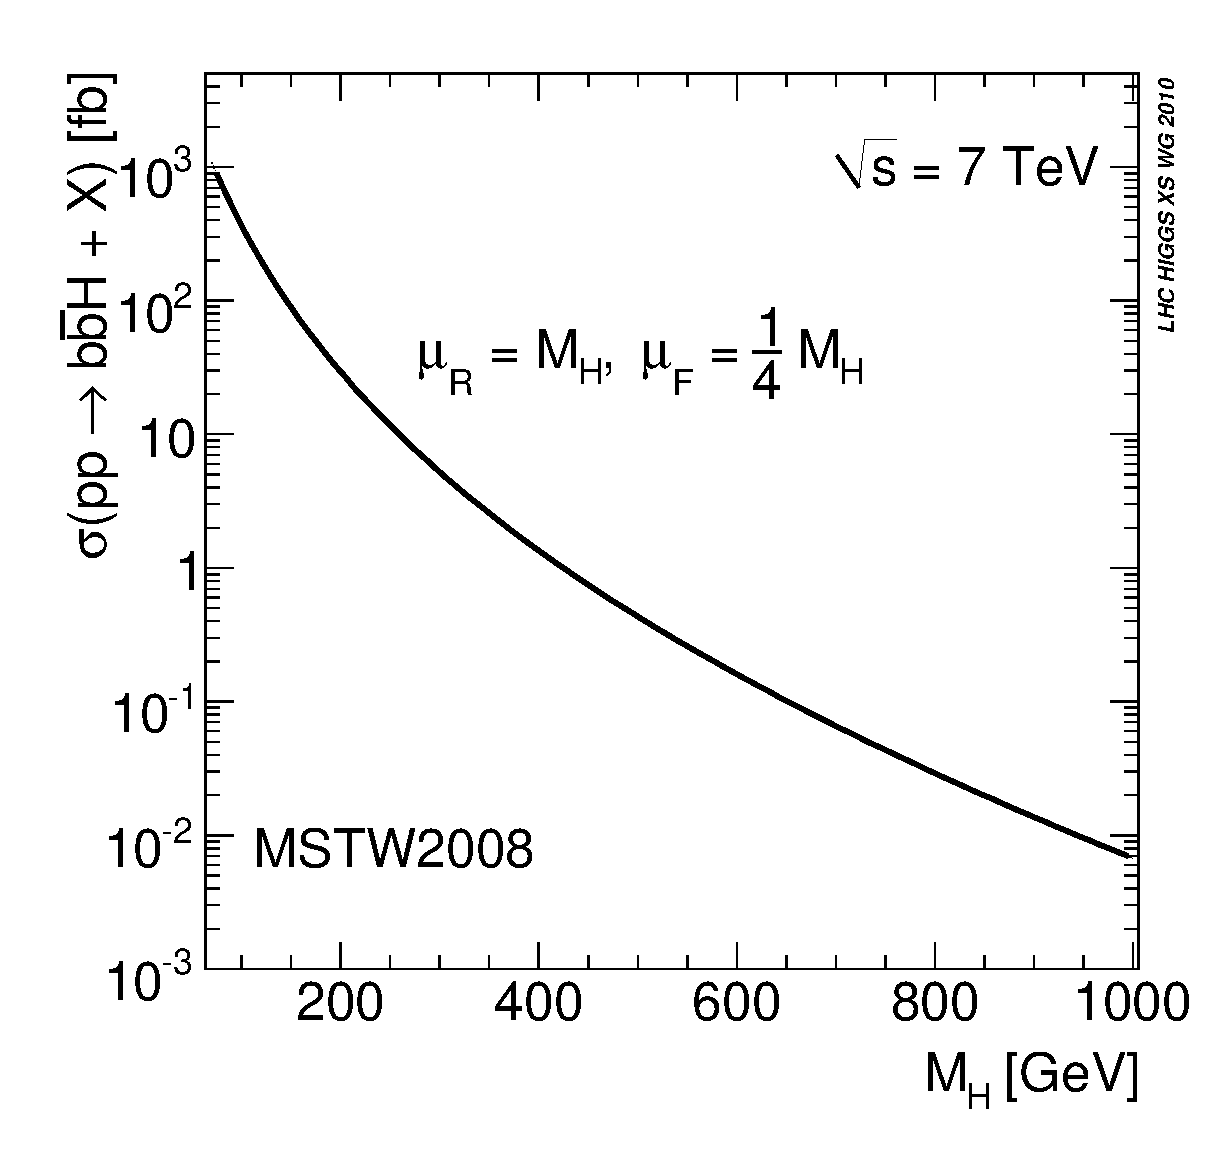
\includegraphics[width=0.5\textwidth]{YRHXS_MSSM_neutral/YRHXS_MSSM_neutral_fig4a.eps}}
\subfigure[]{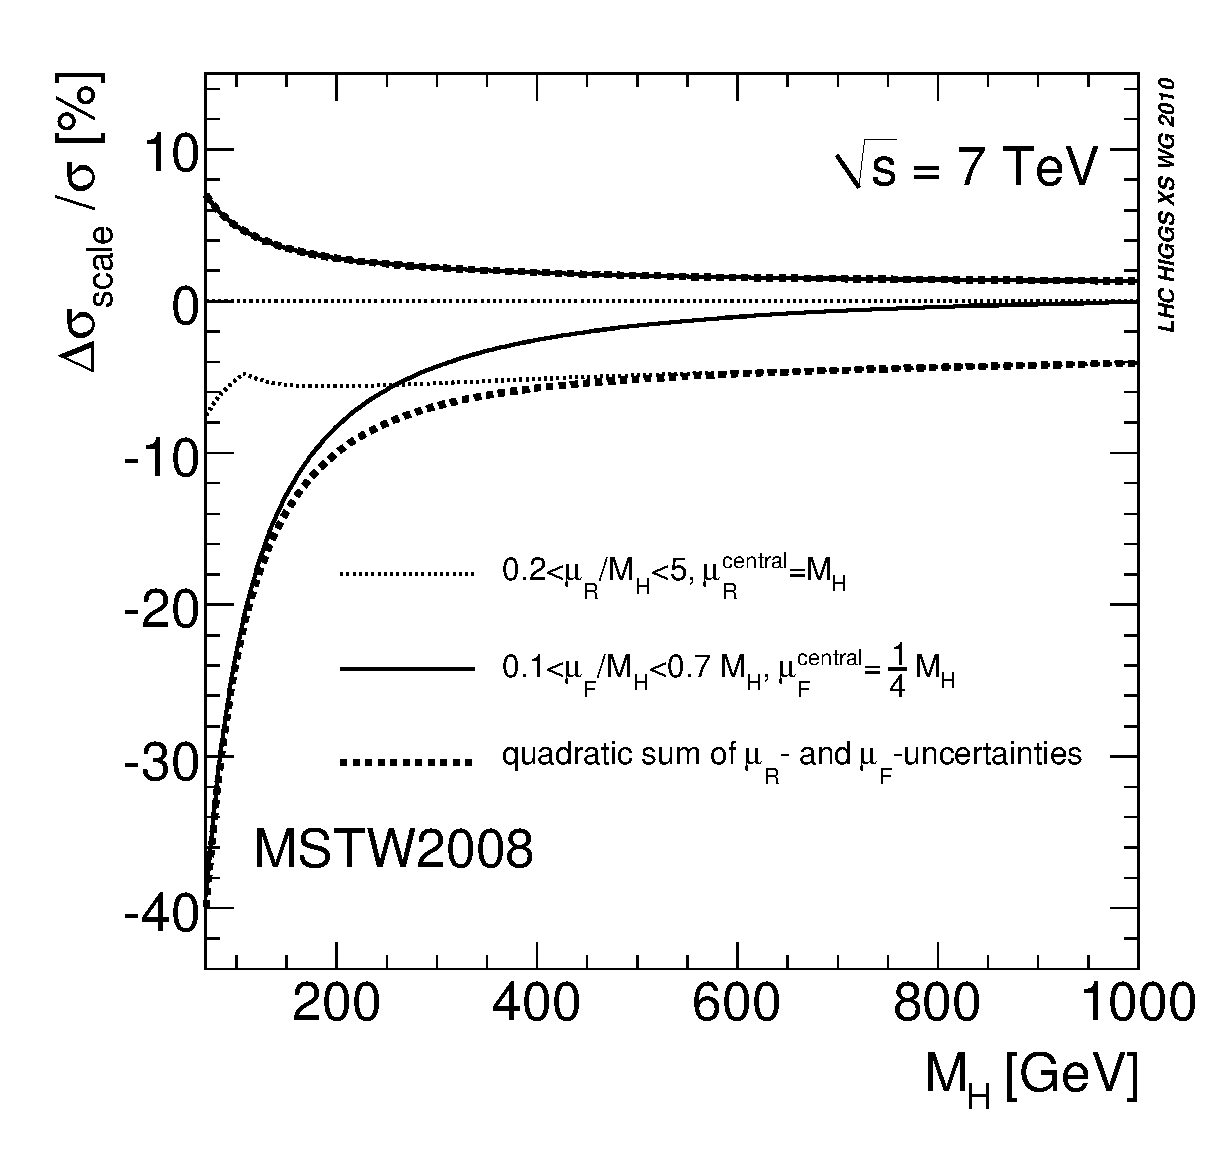
\includegraphics[width=0.5\textwidth]{YRHXS_MSSM_neutral/YRHXS_MSSM_neutral_fig4b.eps}}
\subfigure[]{\includegraphics[width=0.5\textwidth]{YRHXS_MSSM_neutral/YRHXS_MSSM_neutral_fig4c.eps}}
\subfigure[]{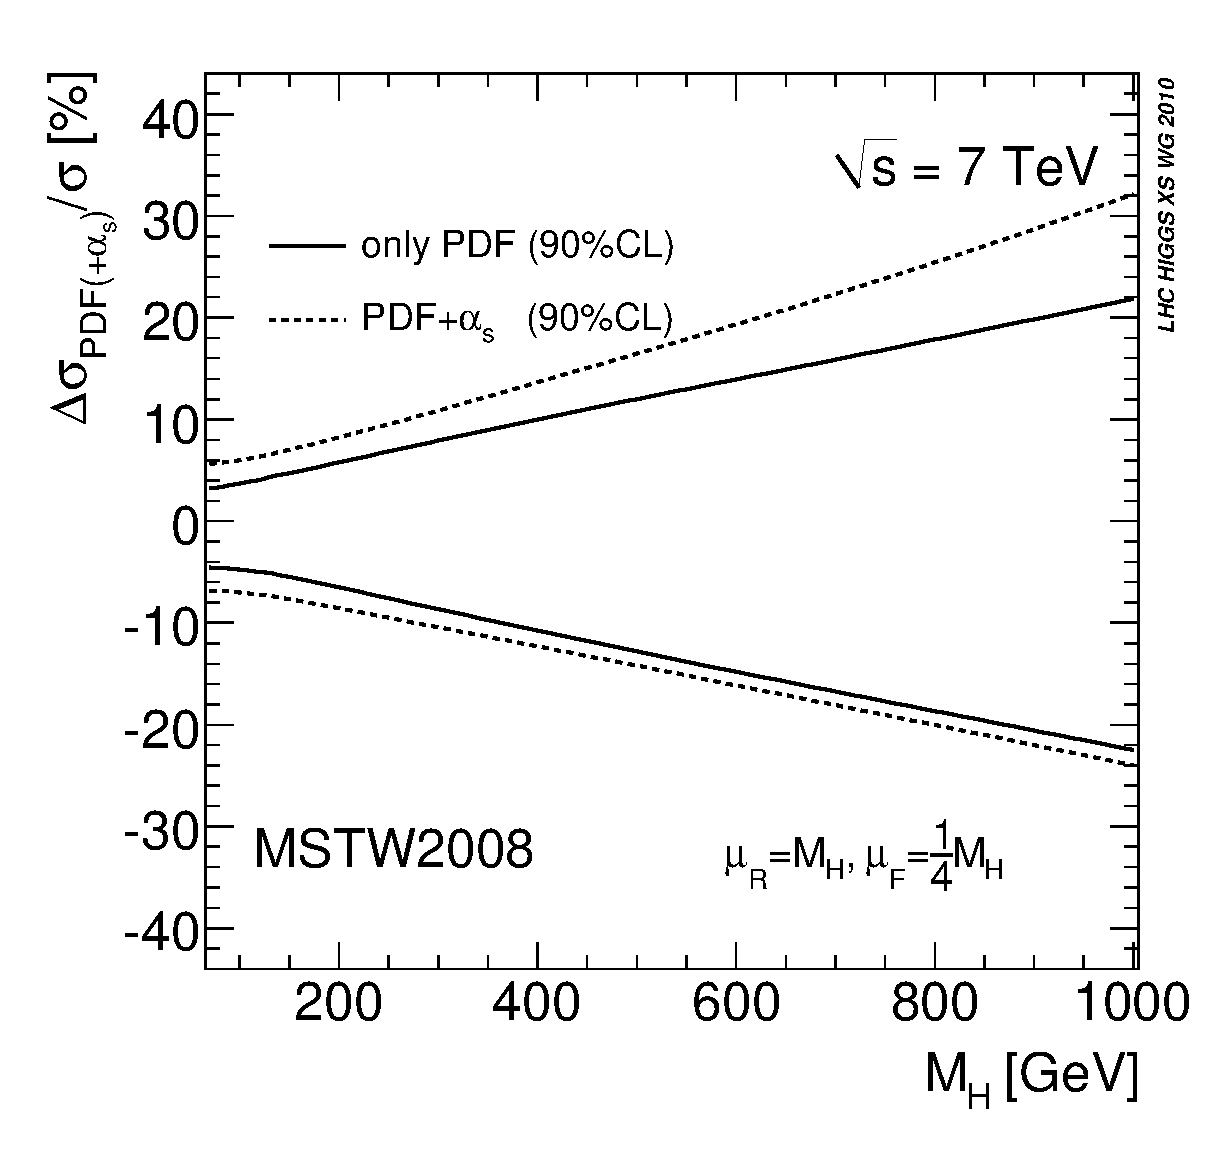
\includegraphics[width=0.5\textwidth]{YRHXS_MSSM_neutral/YRHXS_MSSM_neutral_fig4d.eps}}
%\put(20,0){\includegraphics[scale=0.4]{YRHXS_MSSM_neutral/central.eps}}
%\put(250,0){\includegraphics[scale=0.4]{YRHXS_MSSM_neutral/scaleuncert.eps}}
%\put(20,-220){\includegraphics[scale=0.4]{YRHXS_MSSM_neutral/pdf68.eps}}
%\put(250,-220){\includegraphics[scale=0.4]{YRHXS_MSSM_neutral/pdf90.eps}}
%\put(130,5){$(a)$}
%\put(370,5){$(b)$}
%\put(130,-215){$(c)$}
%\put(370,-215){$(d)$}
%\end{picture} \\[7.0cm]
\caption{\label{YRHXS_MSSM_neutral_fig4} Total bottom-quark-fusion
cross sections of $\PQb\PAQb\to \PSH/\PSA+X$ within the 5FS for $\sqrt{s}=7$\UTeV\ with SM-like couplings using MSTW2008 PDFs
\cite{Martin:2009iq,Martin:2009bu}; (a) central prediction, (b) scale
uncertainties, (c) 68\% CL~PDF+$\alphas$ uncertainties, (d) 90\%
CL~PDF+$\alphas$ uncertainties.}
\end{figure}

In the corresponding 4FS calculation we have chosen the bottom-quark
pole mass as $\Mb=4.75$\UGeV~which corresponds to a NLO 
$\MSbar$
%$\overline{\rm MS}$ 
mass $\overline{m}_\PQb(\overline{m}_\PQb)=4.40$\UGeV. The closed top loop
contributions appearing in the virtual one-loop contributions have been
neglected for consistency, since for large values of $\tanb$ they
are strongly suppressed and in the 5FS calculation they vanish for
strictly massless bottom quarks. In the further progress of this study
we will generate separate grids for these top loop contributions so that
they can be included in the MSSM calculations consistently. The running
bottom-quark Yukawa coupling, expressed in terms of the $\overline{\rm
MS}$ bottom mass, has been chosen at the scale of the Higgs mass
$M_\phi$. The central scales $\mu_R=\mu_F=M_\phi/4$ have been adopted
for the renormalization and factorization scales, respectively. The
scale uncertainties have been obtained for scale variations
$M_\phi/8 < \mu_R,\mu_F < M_\phi/2$ where the choice $\mu_R=\mu_F =
M_\phi/8$ corresponds to the maximal cross sections and $\mu_R=\mu_F =
M_\phi/2$ to the minimal cross sections for all Higgs masses. The
four-flavour PDFs of MSTW2008 \cite{Martin:2010db} have been used for
the numerical analysis within the 4FS. Error PDFs within this scheme
have only been published very recently so that a full PDF uncertainty
analysis could not be performed for the 4FS yet.  However, the scale
uncertainties of $25{-}30\%$ are expected to dominate the overall
uncertainties of the 4FS calculation so that the additional
PDF+$\alphas$ uncertainties will be expected to modify the overall
uncertainties only mildly. The comparison of the 4FS and the 5FS for
SM-like couplings is shown in \Fref{YRHXS_MSSM_neutral_fig5} for
scalar and pseudoscalar Higgs-boson production in association with
bottom quarks.  The scalar and pseudoscalar cross sections for the same
mass differ by less than $2\%$ within the 4FS thanks to the approximate
chiral symmetry for the light bottom quarks compared to the Higgs-boson
masses.  \Fref{YRHXS_MSSM_neutral_fig5} shows good agreement of the
5FS and 4FS results for smaller Higgs masses while for large Higgs-boson
masses the 5FS cross sections are considerably larger than the
corresponding 4FS results. However, an overlap of both uncertainty bands
is visible for the whole mass range. This is the first completely
consistent comparison of both schemes resulting in a much better
agreement of both schemes than in all former studies
\cite{Campbell:2004pu}. The central values of the 4FS and 5FS differ by
up to $30\%$. In order to decide which of the two prescriptions is closer
to the experimentally relevant values of these production cross
sections, the comparison of the 4FS and 5FS calculations of $\PQb\PAQb{+}\PZ$
production with the forthcoming experimental data will be of big help.
\begin{figure}[htb]
%\begin{picture}(130,250)(30,0)
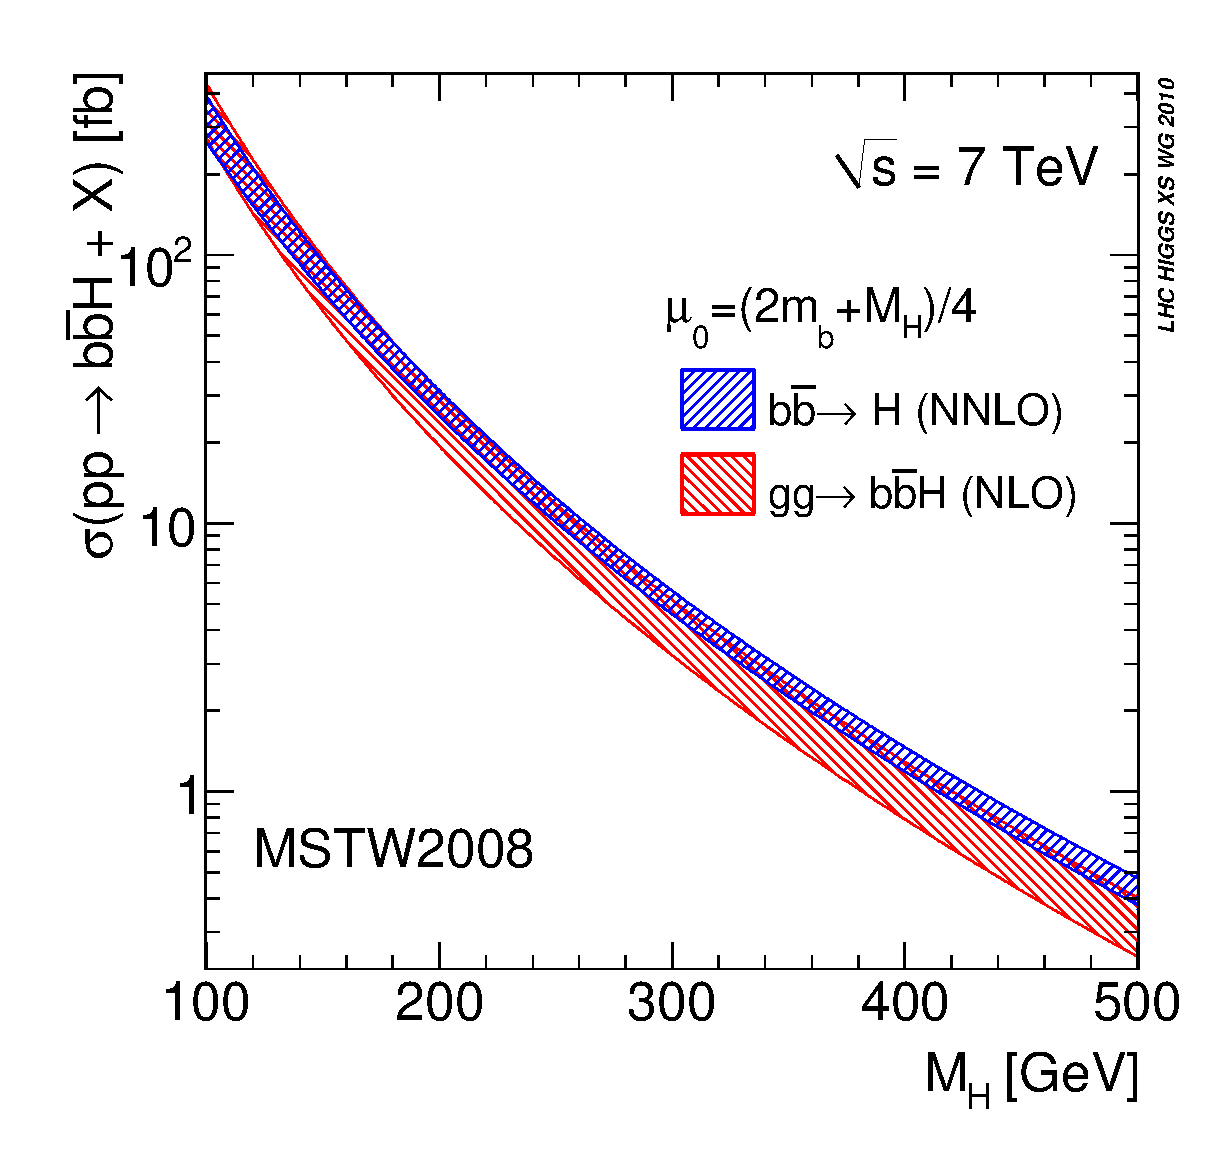
\includegraphics[width=0.5\textwidth]{YRHXS_MSSM_neutral/YRHXS_MSSM_neutral_fig5a.eps}
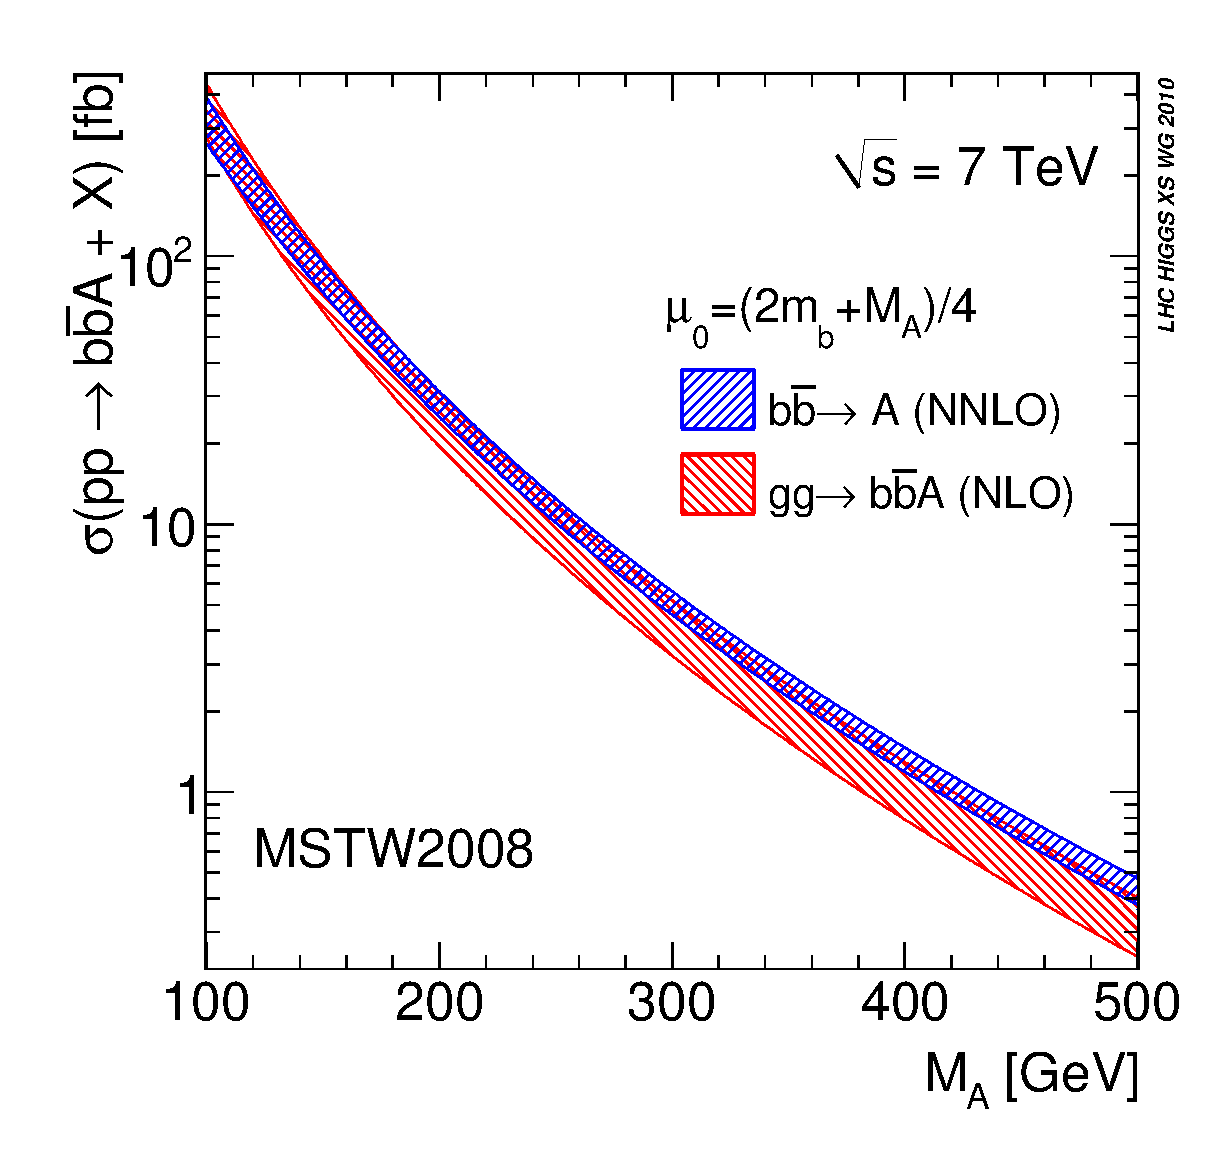
\includegraphics[width=0.5\textwidth]{YRHXS_MSSM_neutral/YRHXS_MSSM_neutral_fig5b.eps}
%\put(80,10){\includegraphics[scale=0.5]{YRHXS_MSSM_neutral/bbh.eps}}
%\put(80,-260){\includegraphics[scale=0.5]{YRHXS_MSSM_neutral/bba.eps}}
%\end{picture} \\[8.3cm]
\caption{\label{YRHXS_MSSM_neutral_fig5} Total production cross
sections of $\Pp\Pp\to \PQb\PAQb\PSH/\PSA+X$ for $\sqrt{s}=7$
\UTeV~within the 5FS and the 4FS using MSTW2008 PDFs
\cite{Martin:2009iq,Martin:2009bu}. The upper bands (blue bands) exhibit the combined
scale and 68\% CL~PDF+$\alphas$ uncertainties of the 5FS, while the
lower bands (red
bands) include the scale uncertainties of the 4FS only.} \end{figure}

In \Fref{YRHXS_MSSM_neutral_fig6} the central predictions for the
gluon-fusion processes $\Pg\Pg\to \PSh,\PSH,\PSA$ and neutral Higgs
radiation off bottom quarks within the 5FS are shown as a function of
the corresponding Higgs mass within the $\mhmaxx$ scenario for two
values of $\tanb=5,30$. These results have been obtained from the grids
generated by \gghnnlo~and \HIGLU~for the gluon-fusion process and
\bbhnnlo~for $\PQb\PAQb\to \phi$ and rescaling the corresponding Yukawa
couplings by the MSSM factors calculated with 
\FeynHiggs{}\footnote{Two complete scans of the ($M_{\PA},\tan\beta)$ 
plane for $\sqrt{s}=7$ and $14$\UTeV\ are available in electronic format 
on {\tt https://twiki.cern.ch/twiki/bin/view/LHCPhysics/MSSMNeutral} 
for the \mhmaxx scenario.}. It is clearly
visible that Higgs-boson radiation off bottom quarks plays the dominant
role for $\tanb=30$ while for $\tanb=5$ the gluon fusion is either
dominant or competitive.
\begin{figure}[htb]
%\begin{picture}(130,250)(30,0)
\subfigure[]{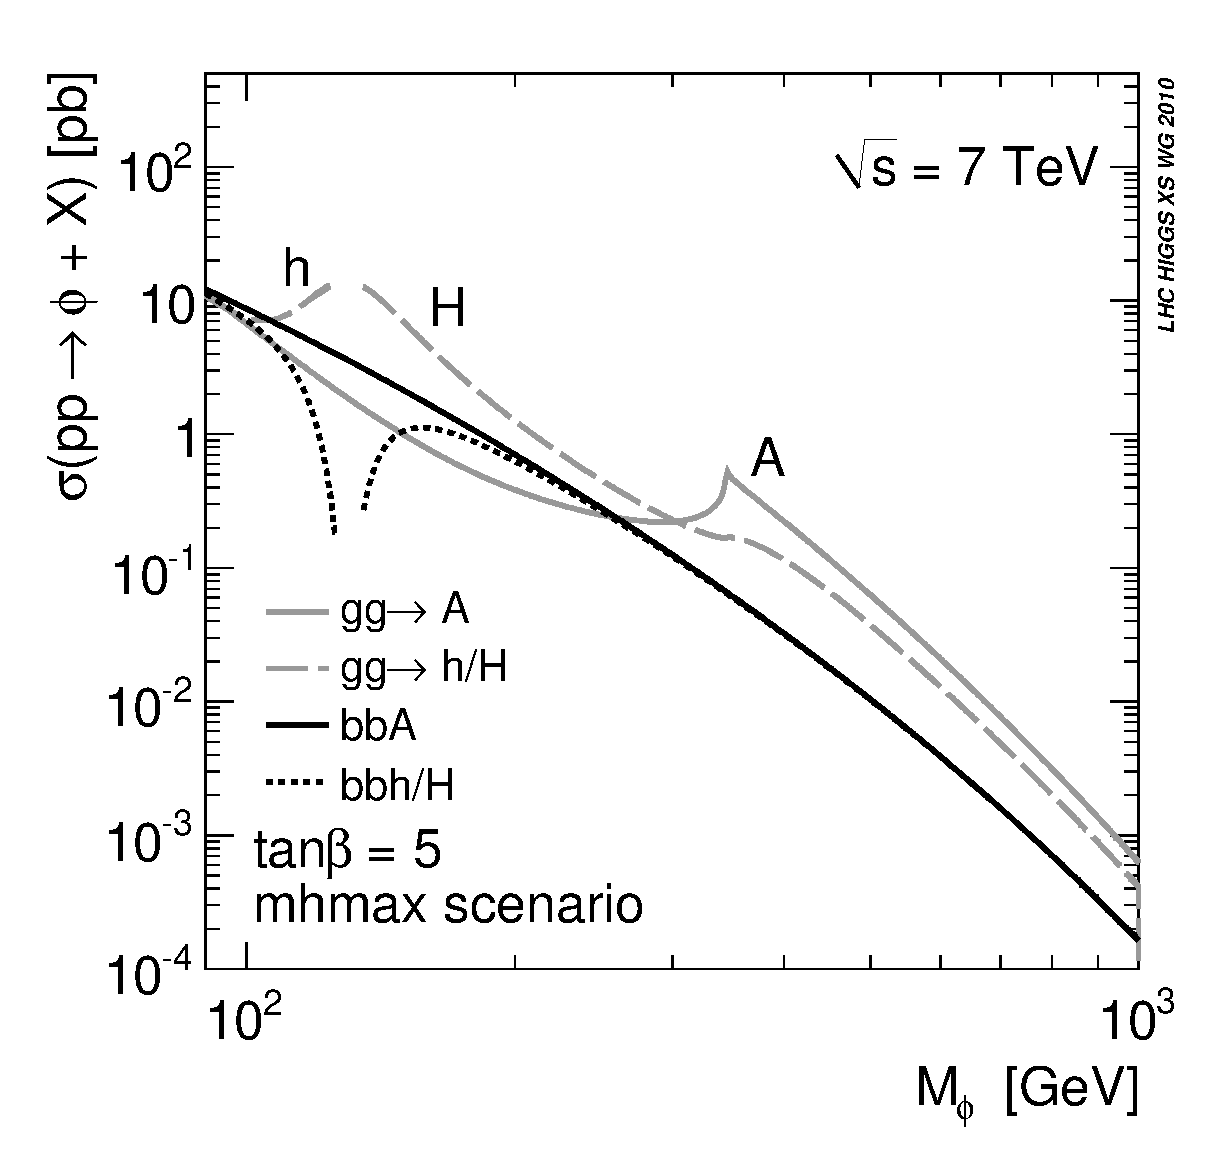
\includegraphics[width=0.5\textwidth]{YRHXS_MSSM_neutral/YRHXS_MSSM_neutral_fig6a.eps}}
\subfigure[]{\includegraphics[width=0.5\textwidth]{YRHXS_MSSM_neutral/YRHXS_MSSM_neutral_fig6b.eps}}
%\end{picture} \\[8.0cm]
\caption{\label{YRHXS_MSSM_neutral_fig6} Central predictions for the
total MSSM production cross sections via gluon fusion and Higgs radiation off
bottom quarks within the 5FS for $\sqrt{s}=7$\UTeV\ using NNLO and NLO
MSTW2008 PDFs \cite{Martin:2009iq,Martin:2009bu} for the $\mhmaxx$
scenario; (a) $\tanb=5$, (b) $\tanb=30$.}
\end{figure}

\clearpage
